% Options for packages loaded elsewhere
\PassOptionsToPackage{unicode}{hyperref}
\PassOptionsToPackage{hyphens}{url}
%
\documentclass[
  11pt]{report}
\usepackage{amsmath,amssymb}
\usepackage{lmodern}
\usepackage{iftex}
\ifPDFTeX
  \usepackage[T1]{fontenc}
  \usepackage[utf8]{inputenc}
  \usepackage{textcomp} % provide euro and other symbols
\else % if luatex or xetex
  \usepackage{unicode-math}
  \defaultfontfeatures{Scale=MatchLowercase}
  \defaultfontfeatures[\rmfamily]{Ligatures=TeX,Scale=1}
\fi
% Use upquote if available, for straight quotes in verbatim environments
\IfFileExists{upquote.sty}{\usepackage{upquote}}{}
\IfFileExists{microtype.sty}{% use microtype if available
  \usepackage[]{microtype}
  \UseMicrotypeSet[protrusion]{basicmath} % disable protrusion for tt fonts
}{}
\makeatletter
\@ifundefined{KOMAClassName}{% if non-KOMA class
  \IfFileExists{parskip.sty}{%
    \usepackage{parskip}
  }{% else
    \setlength{\parindent}{0pt}
    \setlength{\parskip}{6pt plus 2pt minus 1pt}}
}{% if KOMA class
  \KOMAoptions{parskip=half}}
\makeatother
\usepackage{xcolor}
\IfFileExists{xurl.sty}{\usepackage{xurl}}{} % add URL line breaks if available
\IfFileExists{bookmark.sty}{\usepackage{bookmark}}{\usepackage{hyperref}}
\hypersetup{
  pdftitle={Probabilidade e Estatística com R},
  pdfauthor={Fernando Náufel},
  pdflang={pt-br},
  hidelinks,
  pdfcreator={LaTeX via pandoc}}
\urlstyle{same} % disable monospaced font for URLs
\usepackage[margin=1in]{geometry}
\usepackage{color}
\usepackage{fancyvrb}
\newcommand{\VerbBar}{|}
\newcommand{\VERB}{\Verb[commandchars=\\\{\}]}
\DefineVerbatimEnvironment{Highlighting}{Verbatim}{commandchars=\\\{\}}
% Add ',fontsize=\small' for more characters per line
\usepackage{framed}
\definecolor{shadecolor}{RGB}{248,248,248}
\newenvironment{Shaded}{\begin{snugshade}}{\end{snugshade}}
\newcommand{\AlertTok}[1]{\textcolor[rgb]{0.94,0.16,0.16}{#1}}
\newcommand{\AnnotationTok}[1]{\textcolor[rgb]{0.56,0.35,0.01}{\textbf{\textit{#1}}}}
\newcommand{\AttributeTok}[1]{\textcolor[rgb]{0.77,0.63,0.00}{#1}}
\newcommand{\BaseNTok}[1]{\textcolor[rgb]{0.00,0.00,0.81}{#1}}
\newcommand{\BuiltInTok}[1]{#1}
\newcommand{\CharTok}[1]{\textcolor[rgb]{0.31,0.60,0.02}{#1}}
\newcommand{\CommentTok}[1]{\textcolor[rgb]{0.56,0.35,0.01}{\textit{#1}}}
\newcommand{\CommentVarTok}[1]{\textcolor[rgb]{0.56,0.35,0.01}{\textbf{\textit{#1}}}}
\newcommand{\ConstantTok}[1]{\textcolor[rgb]{0.00,0.00,0.00}{#1}}
\newcommand{\ControlFlowTok}[1]{\textcolor[rgb]{0.13,0.29,0.53}{\textbf{#1}}}
\newcommand{\DataTypeTok}[1]{\textcolor[rgb]{0.13,0.29,0.53}{#1}}
\newcommand{\DecValTok}[1]{\textcolor[rgb]{0.00,0.00,0.81}{#1}}
\newcommand{\DocumentationTok}[1]{\textcolor[rgb]{0.56,0.35,0.01}{\textbf{\textit{#1}}}}
\newcommand{\ErrorTok}[1]{\textcolor[rgb]{0.64,0.00,0.00}{\textbf{#1}}}
\newcommand{\ExtensionTok}[1]{#1}
\newcommand{\FloatTok}[1]{\textcolor[rgb]{0.00,0.00,0.81}{#1}}
\newcommand{\FunctionTok}[1]{\textcolor[rgb]{0.00,0.00,0.00}{#1}}
\newcommand{\ImportTok}[1]{#1}
\newcommand{\InformationTok}[1]{\textcolor[rgb]{0.56,0.35,0.01}{\textbf{\textit{#1}}}}
\newcommand{\KeywordTok}[1]{\textcolor[rgb]{0.13,0.29,0.53}{\textbf{#1}}}
\newcommand{\NormalTok}[1]{#1}
\newcommand{\OperatorTok}[1]{\textcolor[rgb]{0.81,0.36,0.00}{\textbf{#1}}}
\newcommand{\OtherTok}[1]{\textcolor[rgb]{0.56,0.35,0.01}{#1}}
\newcommand{\PreprocessorTok}[1]{\textcolor[rgb]{0.56,0.35,0.01}{\textit{#1}}}
\newcommand{\RegionMarkerTok}[1]{#1}
\newcommand{\SpecialCharTok}[1]{\textcolor[rgb]{0.00,0.00,0.00}{#1}}
\newcommand{\SpecialStringTok}[1]{\textcolor[rgb]{0.31,0.60,0.02}{#1}}
\newcommand{\StringTok}[1]{\textcolor[rgb]{0.31,0.60,0.02}{#1}}
\newcommand{\VariableTok}[1]{\textcolor[rgb]{0.00,0.00,0.00}{#1}}
\newcommand{\VerbatimStringTok}[1]{\textcolor[rgb]{0.31,0.60,0.02}{#1}}
\newcommand{\WarningTok}[1]{\textcolor[rgb]{0.56,0.35,0.01}{\textbf{\textit{#1}}}}
\usepackage{longtable,booktabs,array}
\usepackage{calc} % for calculating minipage widths
% Correct order of tables after \paragraph or \subparagraph
\usepackage{etoolbox}
\makeatletter
\patchcmd\longtable{\par}{\if@noskipsec\mbox{}\fi\par}{}{}
\makeatother
% Allow footnotes in longtable head/foot
\IfFileExists{footnotehyper.sty}{\usepackage{footnotehyper}}{\usepackage{footnote}}
\makesavenoteenv{longtable}
\usepackage{graphicx}
\makeatletter
\def\maxwidth{\ifdim\Gin@nat@width>\linewidth\linewidth\else\Gin@nat@width\fi}
\def\maxheight{\ifdim\Gin@nat@height>\textheight\textheight\else\Gin@nat@height\fi}
\makeatother
% Scale images if necessary, so that they will not overflow the page
% margins by default, and it is still possible to overwrite the defaults
% using explicit options in \includegraphics[width, height, ...]{}
\setkeys{Gin}{width=\maxwidth,height=\maxheight,keepaspectratio}
% Set default figure placement to htbp
\makeatletter
\def\fps@figure{htbp}
\makeatother
% Make links footnotes instead of hotlinks:
\DeclareRobustCommand{\href}[2]{#2\footnote{\url{#1}}}
\setlength{\emergencystretch}{3em} % prevent overfull lines
\providecommand{\tightlist}{%
  \setlength{\itemsep}{0pt}\setlength{\parskip}{0pt}}
\setcounter{secnumdepth}{5}
\ifLuaTeX
\usepackage[bidi=basic]{babel}
\else
\usepackage[bidi=default]{babel}
\fi
\babelprovide[main,import]{brazilian}
% get rid of language-specific shorthands (see #6817):
\let\LanguageShortHands\languageshorthands
\def\languageshorthands#1{}

\hypersetup{
  colorlinks,
  breaklinks
}

% Lexend font
\usepackage{lexend}


% Para bibliografia em português
\usepackage{babelbib}

% Para títulos de capítulos e seções:
\usepackage[nobottomtitles*]{titlesec}

%%%%%%%%%%%%%%%
%
% Titulos de capítulos e seções

\titleformat{\chapter}[display]%
{\bfseries\Large}%
{\filleft\MakeUppercase{\chaptertitlename} \Huge\thechapter}%
{4ex}%
{\titlerule%
  \vspace{2ex}%
  \filright}%
[\vspace{2ex}%
\titlerule%
\vspace{10ex}]

\titleformat{\section}[block]%
{\bfseries\Large}%
{\thesection}{.5em}{\titlerule\\[.8ex]\bfseries}

\titleformat{\subsection}[block]%
{\bfseries}%
{\thesubsection}{.5em}{\titlerule\\[.8ex]\bfseries}


%%%%%%%%%%%%%%%
%
% Caixas

\usepackage{tcolorbox}

\tcbset{
  rounded corners,
  boxrule=0.3mm,
  colback=black!.5!white,
  parbox=false
}

\newtcolorbox{rmdbox}{
  colframe=black!40!white,
}


\newtcolorbox{mycaution}{
  colframe=red!75!black,
  sidebyside,
  lower separated=false,
  lefthand width=1cm,
  sidebyside gap=4mm
}

\newenvironment{rmdcaution}
{
  \begin{mycaution}
    
\includegraphics{images/caution.png}
    \tcblower
  }
  {
  \end{mycaution}
}

\newtcolorbox{myimportant}{
  colframe=green!75!black,
  sidebyside,
  lower separated=false,
  lefthand width=1cm,
  sidebyside gap=4mm
}

\newenvironment{rmdimportant}
{
  \begin{myimportant}
    
\includegraphics{images/important.png}
    \tcblower
  }
  {
  \end{myimportant}
}

\newtcolorbox{mywarning}{
  colframe=yellow!80!black,
  sidebyside,
  lower separated=false,
  lefthand width=1cm,
  sidebyside gap=4mm
}

\newenvironment{rmdwarning}
{
  \begin{mywarning}
    
\includegraphics{images/warning.png}
    \tcblower
  }
  {
  \end{mywarning}
}

\newtcolorbox{mynote}{
  colframe=yellow!70!black,
  sidebyside,
  lower separated=false,
  lefthand width=1cm,
  sidebyside gap=4mm
}

\newenvironment{rmdnote}
{
  \begin{mynote}
    
\includegraphics{images/note.png}
    \tcblower
  }
  {
  \end{mynote}
}

\newtcolorbox{mytip}{
  colframe=blue!50!white,
  sidebyside,
  lower separated=false,
  lefthand width=1cm,
  sidebyside gap=4mm
}

\newenvironment{rmdtip}
{
  \begin{mytip}
    
\includegraphics{images/tip.png}
    \tcblower
  }
  {
  \end{mytip}
}

% For highlighting using \hl{}
\usepackage{soul}
\usepackage{booktabs}
\usepackage{longtable}
\usepackage{array}
\usepackage{multirow}
\usepackage{wrapfig}
\usepackage{float}
\usepackage{colortbl}
\usepackage{pdflscape}
\usepackage{tabu}
\usepackage{threeparttable}
\usepackage{threeparttablex}
\usepackage[normalem]{ulem}
\usepackage{makecell}
\usepackage{xcolor}
\ifLuaTeX
  \usepackage{selnolig}  % disable illegal ligatures
\fi
\usepackage[]{natbib}
\bibliographystyle{apalike}

\title{Probabilidade e Estatística com R}
\author{Fernando Náufel}
\date{(versão de 11/11/2021)}

\begin{document}
\maketitle

{
\setcounter{tocdepth}{1}
\tableofcontents
}
\hypertarget{apresentacao}{%
\chapter*{Apresentação}\label{apresentacao}}
\addcontentsline{toc}{chapter}{Apresentação}

\begin{rmdcaution}
\textbf{Atenção}

Este material ainda está em construção.

Pode haver mudanças a qualquer momento.

Verifique, no rodapé da página \emph{web} ou na capa do arquivo pdf, a data desta versão.

\end{rmdcaution}

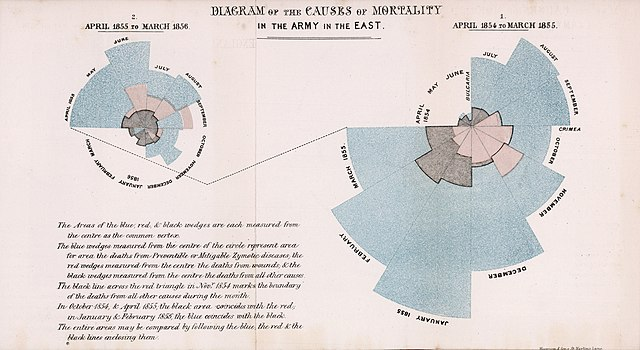
\includegraphics{images/640px-Nightingale-mortality.jpg}

Este livro/site foi iniciado em 2020, durante a pandemia de COVID-19, quando a Universidade Federal Fluminense (UFF) funcionou em regime de ensino remoto durante mais de um ano.

Para atender os alunos do curso de Probabilidade e Estatística do curso de graduação em Ciência da Computação da UFF, decidi gravar aulas em vídeo e disponibilizar os arquivos usados nelas. Foram esses arquivos que deram origem a este livro/site.

Para tirar o máximo proveito deste material, você deve fazer o seguinte:

\begin{enumerate}
\def\labelenumi{\arabic{enumi}.}
\item
  Assistir aos vídeos contidos em cada capítulo. A \emph{playlist} completa está em \url{https://www.youtube.com/playlist?list=PL7SRLwLs7ocaV-Y1vrVU3W7mZnnS0qkWV}.
\item
  Instalar o R no seu computador ou abrir uma conta no RStudio Cloud, para poder usar o R \emph{online}. Você encontra instruções para fazer isto no \protect\hyperlink{rintro}{capítulo de introdução a R}.
\item
  Seguir os \emph{links} para outras fontes \emph{online} que abordam assuntos que não são cobertos em detalhes neste curso.
\item
  Fazer os exercícios. Ao longo do tempo, acrescentarei \emph{links} para vídeos explicando as soluções.
\end{enumerate}

O código-fonte deste livro/site pode ser encontrado \href{https://github.com/fnaufel/probestr}{neste repositório do Github}.

Se você preferir ler este livro em pdf, ou se quiser imprimi-lo, \href{https://github.com/fnaufel/probestr/blob/master/docs/probestr.pdf}{faça o download do arquivo aqui}.

\hypertarget{exercuxedcio}{%
\section*{Exercício}\label{exercuxedcio}}
\addcontentsline{toc}{section}{Exercício}

\begin{enumerate}
\def\labelenumi{\arabic{enumi}.}
\tightlist
\item
  Pesquise sobre a imagem do início deste capítulo. Ela foi criada em 1858 por Florence Nightingale.
\end{enumerate}

\hypertarget{oque}{%
\chapter{O Que É Estatística?}\label{oque}}

\hypertarget{vuxeddeo-1}{%
\section{Vídeo 1}\label{vuxeddeo-1}}

\begin{center} \url{https://youtu.be/6Q_XSoLCIpc} \end{center}

\hypertarget{exercuxedcios}{%
\section{Exercícios}\label{exercuxedcios}}

\begin{enumerate}
\def\labelenumi{\arabic{enumi}.}
\item
  Você está interessado em estimar a altura de todos os homens da sua faculdade. Para isso, você decide medir as alturas de todos os homens da sua turma de Estatística.

  \begin{itemize}
  \tightlist
  \item
    Qual é a amostra?
  \item
    Qual é a população?
  \end{itemize}
\item
  Um instituto de pesquisa entrevista um grupo de \(1000\) pessoas, perguntando a cada uma se ela vai votar a favor do candidato \(A\) na próxima eleição. Dos entrevistados, \(600\) responderam que sim. A proporção \(0{,}6\) (ou \(60\%\)) é uma estatística ou um parâmetro?
\item
  Você vê alguma diferença entre as cinco situações abaixo? Quais das situações são equivalentes em termos da probabilidade de conseguir \(5\) cartas do mesmo naipe?

  \begin{enumerate}
  \def\labelenumii{\alph{enumii}.}
  \item
    Usando um baralho normal, você retira \(10\) cartas e registra as cartas retiradas.
  \item
    Usando um baralho normal, você repete a seguinte sequência de ações \(10\) vezes: retirar uma carta do baralho, registrar a carta retirada e repor a carta no baralho.
  \item
    Usando uma caixa contendo todas as cartas de \(1\) milhão de baralhos reunidos, você retira \(10\) cartas e registra as cartas retiradas.
  \item
    Usando uma caixa contendo todas as cartas de \(1\) milhão de baralhos reunidos, você repete a seguinte sequência de ações \(10\) vezes: retirar uma carta da caixa, registrar a carta retirada e repor a carta na caixa.
  \item
    Usando um baralho \emph{infinito}, você retira \(10\) cartas e registra as cartas retiradas.
  \item
    Usando um baralho \emph{infinito}, você repete a seguinte sequência de ações \(10\) vezes: retirar uma carta do baralho, registrar a carta retirada e repor a carta no baralho.
  \end{enumerate}
\item
  Qual a graça dos quadrinhos na Figura \ref{fig:xkcd-cor}, que também \href{https://youtu.be/6Q_XSoLCIpc?t=1385}{aparecem no vídeo}?

  \begin{figure}

   {\centering 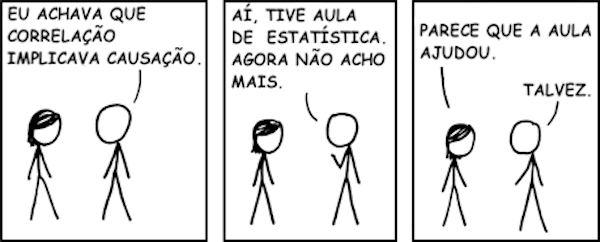
\includegraphics[width=0.9\linewidth]{images/correlation-pt-600} 

   }

   \caption{\url{http://xkcd.com/552/}}\label{fig:xkcd-cor}
   \end{figure}
\item
  Qual a graça dos quadrinhos na Figura \ref{fig:xkcd-blind}?

  \begin{figure}

   {\centering 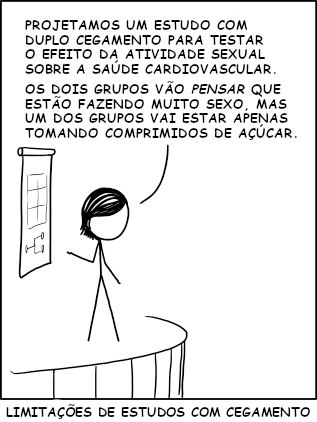
\includegraphics[width=0.5\linewidth]{images/double-blind} 

   }

   \caption{\url{http://xkcd.com/1462/}}\label{fig:xkcd-blind}
   \end{figure}
\item
  Veja este vídeo sobre o cavalo Hans:

  \begin{center} \url{https://youtu.be/G3VkCmdUfZE} \end{center}

  Qual a relação entre esta história e a necessidade de duplo cegamento?
\end{enumerate}





\hypertarget{vuxeddeo-2}{%
\section{Vídeo 2}\label{vuxeddeo-2}}

\begin{center} \url{https://youtu.be/492VASxlDRo} \end{center}

\hypertarget{exercuxedcios-1}{%
\section{Exercícios}\label{exercuxedcios-1}}

\begin{enumerate}
\def\labelenumi{\arabic{enumi}.}
\item
  Por que não faz sentido calcular a média dos CEPs de um grupo de pessoas?
\item
  Uma temperatura de \(-40\) graus Celsius é igual a uma temperatura de \(-40\) graus Fahrenheit?
\item
  Uma temperatura de zero graus Celsius é igual a uma temperatura de zero graus Fahrenheit?
\item
  Uma variação de temperatura de \(1\) grau Celsius é igual a uma variação de temperatura de \(1\) grau Fahrenheit?
\item
  Um saldo bancário de zero reais é igual a um saldo bancário de zero dólares?
\item
  Um produto de \(1\) milhão de reais custa o mesmo que um produto de \(1\) milhão de dólares?
\item
  Meses representados por números de \(1\) a \(12\) são dados de que nível?
\end{enumerate}

\hypertarget{rintro}{%
\chapter{Introdução a R}\label{rintro}}

\hypertarget{vuxeddeo-1-1}{%
\section{Vídeo 1}\label{vuxeddeo-1-1}}

\begin{center} \url{https://youtu.be/1kXQDNqm41c} \end{center}

\hypertarget{vuxeddeo-2-1}{%
\section{Vídeo 2}\label{vuxeddeo-2-1}}

\begin{center} \url{https://youtu.be/3GEc1oiKDrU} \end{center}

\hypertarget{exercuxedcios-2}{%
\section{Exercícios}\label{exercuxedcios-2}}

\begin{enumerate}
\def\labelenumi{\arabic{enumi}.}
\item
  Para criar sua conta no RStudio Cloud, acesse \url{https://rstudio.cloud/}.
\item
  Se você preferir instalar o R no seu computador, acesse

  \begin{itemize}
  \item
    \url{https://cran.r-project.org/} para baixar e instalar o R, e
  \item
    \url{https://rstudio.com/products/rstudio/download/} para baixar e instalar o RStudio, um IDE específico para R.
  \end{itemize}
\item
  Abra o RStudio Cloud ou o seu RStudio instalado localmente.
\item
  Crie um novo projeto. {\hl{Sempre trabalhe em projetos para ter seus arquivos organizados.}}
\item
  Para instalar o \href{https://swirlstats.com/}{\texttt{swirl} (pacote do R para exercícios interativos)}, execute o seguinte comando no console do RStudio:

\begin{Shaded}
\begin{Highlighting}[]
\FunctionTok{install.packages}\NormalTok{(}\StringTok{"swirl"}\NormalTok{)}
\end{Highlighting}
\end{Shaded}
\item
  Para instalar os exercícios de introdução a R, execute os seguintes comandos no console do RStudio:

\begin{Shaded}
\begin{Highlighting}[]
\FunctionTok{library}\NormalTok{(swirl)}
\FunctionTok{install\_course\_github}\NormalTok{(}\StringTok{\textquotesingle{}fnaufel\textquotesingle{}}\NormalTok{, }\StringTok{\textquotesingle{}introR\textquotesingle{}}\NormalTok{)}
\end{Highlighting}
\end{Shaded}
\item
  Mude o idioma para português e execute o \texttt{swirl}.

\begin{Shaded}
\begin{Highlighting}[]
\FunctionTok{select\_language}\NormalTok{(}\StringTok{\textquotesingle{}portuguese\textquotesingle{}}\NormalTok{, }\AttributeTok{append\_rprofile =} \ConstantTok{TRUE}\NormalTok{)}
\FunctionTok{swirl}\NormalTok{()}
\end{Highlighting}
\end{Shaded}
\item
  Na primeira execução, você vai precisar se identificar (qualquer nome serve). Com essa identificação, o \texttt{swirl} vai registrar o seu progresso nas lições.
\item
  No \texttt{swirl}, as perguntas são mostradas no console. Você também deve responder no console.
\item
  Às vezes, um \emph{script} será aberto no editor de textos para que você complete um programa. Quando seu programa estiver pronto, salve o arquivo e digite \texttt{submit()} no console para o \texttt{swirl} processar o \emph{script}.
\item
  O \texttt{swirl} dá instruções claras no console. Na dúvida, digite \texttt{info()} no \emph{prompt} do R (\texttt{\textgreater{}}).
\item
  Se, em vez do \emph{prompt} do R, o console mostrar reticências (\texttt{...}), tecle \emph{Enter}.
\item
  Se nada funcionar, tecle \emph{ESC}.
\item
  Para sair do \texttt{swirl()}, digite \texttt{bye()} no \emph{prompt} do R.
\item
  Para voltar para os exercícios, digite

\begin{Shaded}
\begin{Highlighting}[]
\FunctionTok{library}\NormalTok{(swirl)}
\FunctionTok{swirl}\NormalTok{()}
\end{Highlighting}
\end{Shaded}
\end{enumerate}

\hypertarget{viz}{%
\chapter{Visualização com ggplot2}\label{viz}}

\hypertarget{vuxeddeo-1-2}{%
\section{Vídeo 1}\label{vuxeddeo-1-2}}

\begin{center} \url{https://youtu.be/OBpNjqIIyhI} \end{center}

\hypertarget{componentes-de-um-gruxe1fico-ggplot2}{%
\section{Componentes de um gráfico ggplot2}\label{componentes-de-um-gruxe1fico-ggplot2}}

\hypertarget{geometrias-e-mapeamentos-estuxe9ticos-mappings}{%
\subsection{\texorpdfstring{Geometrias e mapeamentos estéticos (\emph{mappings})}{Geometrias e mapeamentos estéticos (mappings)}}\label{geometrias-e-mapeamentos-estuxe9ticos-mappings}}

\begin{itemize}
\tightlist
\item
  Observe o gráfico abaixo, obtido de \url{https://www.gapminder.org/downloads/updated-gapminder-world-poster-2015/}.
\end{itemize}

\begin{center}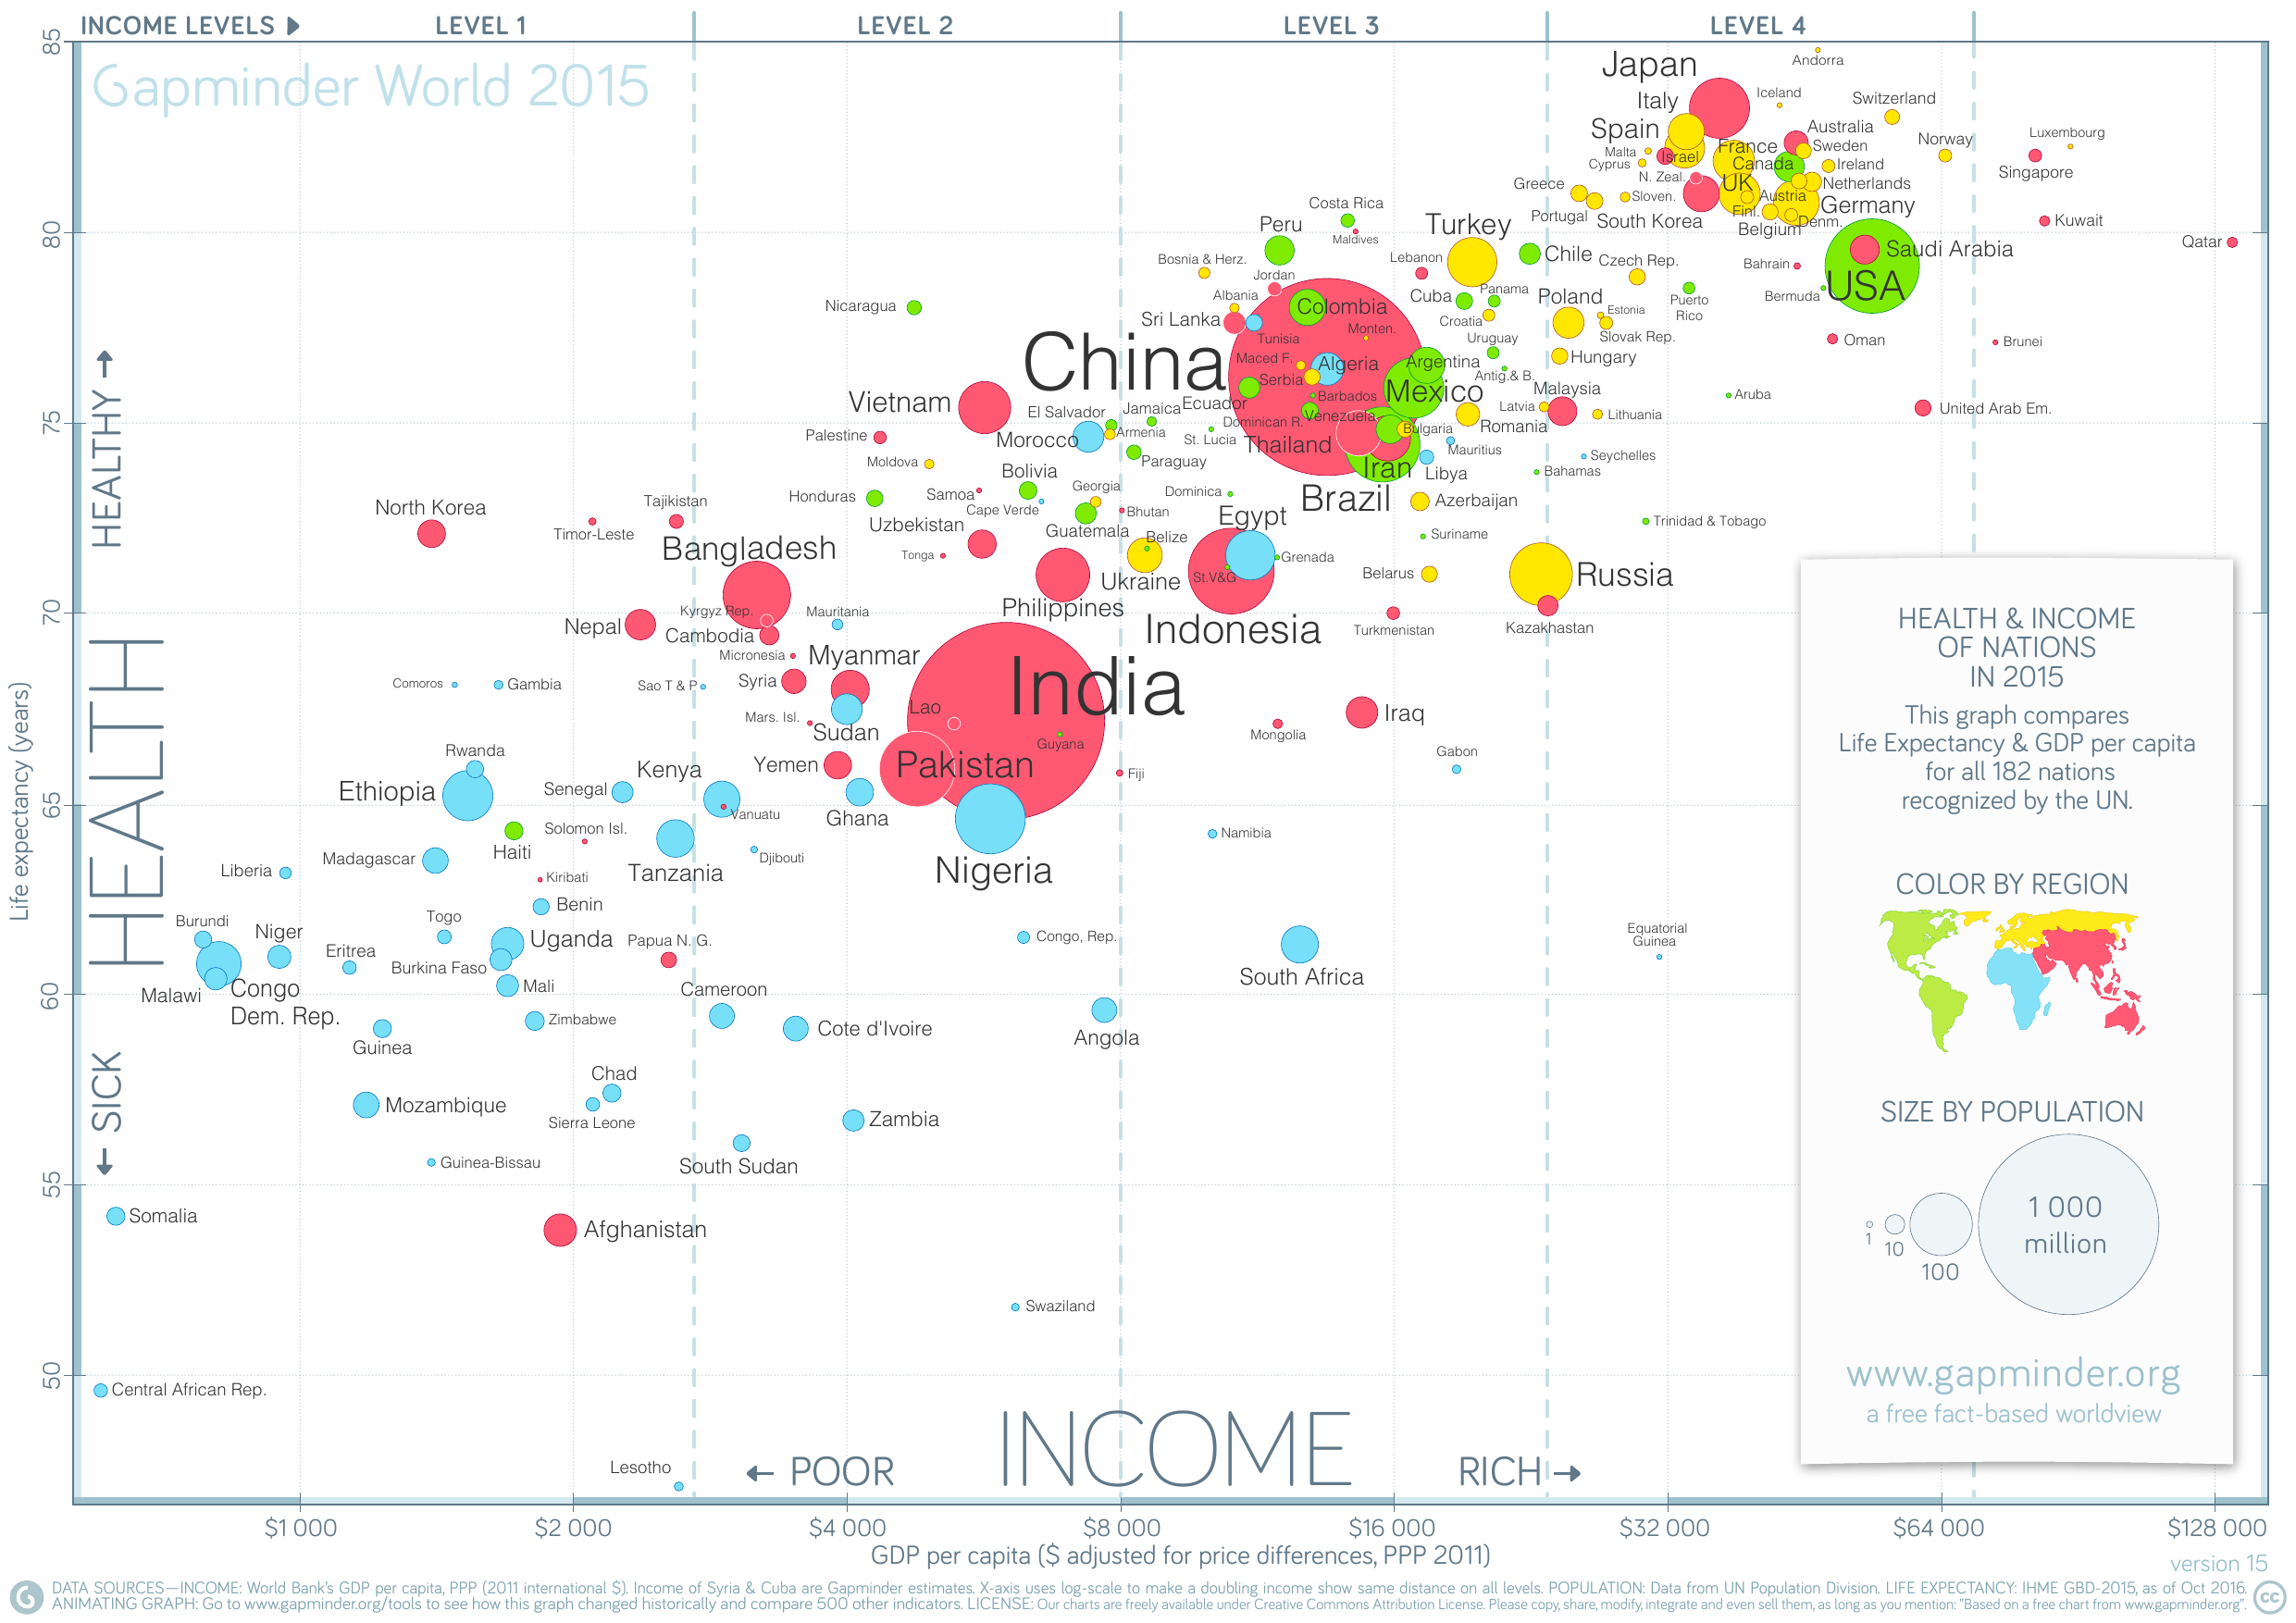
\includegraphics[width=1\linewidth]{images/countries-1} \end{center}

\begin{itemize}
\item
  O gráfico mostra como, em cada país, a saúde (mais precisamente, a expectativa de vida) se relaciona com a riqueza (mais precisamente, o PIB \emph{per capita}).
\item
  Além da expectativa de vida e o do PIB \emph{per capita}, o gráfico traz mais informações sobre cada país.
\item
  Cada país é representado por um ponto (a {\hl{geometria}}).
\item
  Informações sobre cada país são representadas por características do ponto correspondente (as {\hl{estéticas}}):

  \begin{longtable}[]{@{}lll@{}}
  \toprule
  Variável & Geometria & Estética \\
  \midrule
  \endhead
  PIB \emph{per capita} & ponto & posição x \\
  Expectativa de vida & ponto & posição y \\
  População & ponto & tamanho \\
  Continente & ponto & cor \\
  \bottomrule
  \end{longtable}
\item
  Você pode usar outras estéticas para representar informações:

  \begin{itemize}
  \tightlist
  \item
    Cor de preenchimento.
  \item
    Cor do traço.
  \item
    Tipo do traço (sólido, pontilhado, tracejado etc.).
  \item
    Forma (círculo, quadrado, triângulo etc.).
  \item
    Opacidade.
  \item
    etc.
  \end{itemize}
\item
  Você pode usar outras geometrias:

  \begin{itemize}
  \tightlist
  \item
    Linhas.
  \item
    Barras ou colunas.
  \item
    Caixas.
  \item
    etc.
  \end{itemize}
\end{itemize}

\hypertarget{escalas-scales}{%
\subsection{\texorpdfstring{Escalas (\emph{scales})}{Escalas (scales)}}\label{escalas-scales}}

\begin{itemize}
\item
  As escalas controlam os detalhes da aparência da geometria e do mapeamento (eixos, cores etc.).
\item
  Os eixos do gráfico acima são escalas {\hl{contínuas}}, com valores reais.
\item
  Observe o eixo horizontal. Os valores não aumentam linearmente, mas sim exponencialmente: cada passo à direita equivale a \emph{dobrar} o valor do PIB. O eixo horizontal segue uma {\hl{escala logarítmica}}.
\item
  Os tamanhos dos pontos formam uma escala {\hl{discreta}}, com \(4\) valores possíveis (veja a legenda no canto inferior direito do gráfico).
\item
  As cores também formam uma escala discreta.
\end{itemize}

\hypertarget{ruxf3tulos-labels}{%
\subsection{\texorpdfstring{Rótulos (\emph{labels})}{Rótulos (labels)}}\label{ruxf3tulos-labels}}

\begin{itemize}
\item
  O gráfico também representa informação na forma de texto.
\item
  Além de rótulos (por exemplo, o texto que identifica cada eixo), {\hl{o texto também pode, ele mesmo, ser uma geometria, com suas próprias estéticas:}} observe como o nome de cada país é escrito em um tamanho proporcional à sua população.
\end{itemize}

\hypertarget{outros-componentes}{%
\subsection{Outros componentes}\label{outros-componentes}}

\begin{itemize}
\item
  Coordenadas:

  \begin{itemize}
  \item
    Este gráfico usa {\hl{coordenadas cartesianas}}, com eixos \(x\) e \(y\).
  \item
    Existem gráficos que usam um sistema de {\hl{coordenadas polares}}.
  \end{itemize}
\item
  Temas:

  \begin{itemize}
  \item
    Incluem todos os elementos ``decorativos'': cor de fundo, linhas de grade, etc. Ajudam a facilitar a leitura e a interpretação.
  \item
    No gráfico acima, um detalhe interessante do tema é a divisão de cada eixo em segmentos claros e segmentos escuros.
  \end{itemize}
\item
  Legendas (\emph{guides}).
\item
  Facetas:

  \begin{itemize}
  \item
    Às vezes, um gráfico é composto por múltiplos subgráficos.
  \item
    Cada subgráfico é uma {\hl{faceta}}.
  \item
    Facetas evitam que informações demais sejam apresentadas no mesmo lugar.
  \end{itemize}
\end{itemize}

\hypertarget{conjunto-de-dados}{%
\section{Conjunto de dados}\label{conjunto-de-dados}}

\begin{itemize}
\item
  Nossos exemplos de gráficos vão usar dados sobre o sono de diversos mamíferos.
\item
  O conjunto de dados se chama \texttt{msleep} e está incluído no pacote \texttt{ggplot2}.
\item
  Para ver a documentação, digite

\begin{Shaded}
\begin{Highlighting}[]
\FunctionTok{library}\NormalTok{(ggplot2)}
\NormalTok{?msleep}
\end{Highlighting}
\end{Shaded}
\item
  Vamos atribuir o conjunto de dados à variável \texttt{df}:

\begin{Shaded}
\begin{Highlighting}[]
\NormalTok{df }\OtherTok{\textless{}{-}}\NormalTok{ msleep}
\NormalTok{df}
\DocumentationTok{\#\# \# A tibble: 83 x 11}
\DocumentationTok{\#\#   name   genus vore  order conservation sleep\_total sleep\_rem sleep\_cycle}
\DocumentationTok{\#\#   \textless{}chr\textgreater{}  \textless{}chr\textgreater{} \textless{}chr\textgreater{} \textless{}chr\textgreater{} \textless{}chr\textgreater{}              \textless{}dbl\textgreater{}     \textless{}dbl\textgreater{}       \textless{}dbl\textgreater{}}
\DocumentationTok{\#\# 1 Cheet\textasciitilde{} Acin\textasciitilde{} carni Carn\textasciitilde{} lc                  12.1      NA        NA    }
\DocumentationTok{\#\# 2 Owl m\textasciitilde{} Aotus omni  Prim\textasciitilde{} \textless{}NA\textgreater{}                17         1.8      NA    }
\DocumentationTok{\#\# 3 Mount\textasciitilde{} Aplo\textasciitilde{} herbi Rode\textasciitilde{} nt                  14.4       2.4      NA    }
\DocumentationTok{\#\# 4 Great\textasciitilde{} Blar\textasciitilde{} omni  Sori\textasciitilde{} lc                  14.9       2.3       0.133}
\DocumentationTok{\#\# 5 Cow    Bos   herbi Arti\textasciitilde{} domesticated         4         0.7       0.667}
\DocumentationTok{\#\# 6 Three\textasciitilde{} Brad\textasciitilde{} herbi Pilo\textasciitilde{} \textless{}NA\textgreater{}                14.4       2.2       0.767}
\DocumentationTok{\#\# \# ... with 77 more rows, and 3 more variables: awake \textless{}dbl\textgreater{},}
\DocumentationTok{\#\# \#   brainwt \textless{}dbl\textgreater{}, bodywt \textless{}dbl\textgreater{}}
\end{Highlighting}
\end{Shaded}
\item
  Vamos examinar a estrutura --- usando R base:

\begin{Shaded}
\begin{Highlighting}[]
\FunctionTok{str}\NormalTok{(df)}
\DocumentationTok{\#\# tibble [83 x 11] (S3: tbl\_df/tbl/data.frame)}
\DocumentationTok{\#\#  $ name        : chr [1:83] "Cheetah" "Owl monkey" "Mountain beaver" ...}
\DocumentationTok{\#\#  $ genus       : chr [1:83] "Acinonyx" "Aotus" "Aplodontia" ...}
\DocumentationTok{\#\#  $ vore        : chr [1:83] "carni" "omni" "herbi" ...}
\DocumentationTok{\#\#  $ order       : chr [1:83] "Carnivora" "Primates" "Rodentia" ...}
\DocumentationTok{\#\#  $ conservation: chr [1:83] "lc" NA "nt" ...}
\DocumentationTok{\#\#  $ sleep\_total : num [1:83] 12,1 17 14,4 14,9 4 14,4 8,7 7 ...}
\DocumentationTok{\#\#  $ sleep\_rem   : num [1:83] NA 1,8 2,4 2,3 0,7 2,2 1,4 NA ...}
\DocumentationTok{\#\#  $ sleep\_cycle : num [1:83] NA NA NA 0,133 ...}
\DocumentationTok{\#\#  $ awake       : num [1:83] 11,9 7 9,6 9,1 20 9,6 15,3 17 ...}
\DocumentationTok{\#\#  $ brainwt     : num [1:83] NA 0,0155 NA 0,00029 0,423 NA NA NA ...}
\DocumentationTok{\#\#  $ bodywt      : num [1:83] 50 0,48 1,35 0,019 ...}
\end{Highlighting}
\end{Shaded}
\item
  Podemos usar \texttt{glimpse}, uma função do \texttt{tidyverse}:

\begin{Shaded}
\begin{Highlighting}[]
\FunctionTok{glimpse}\NormalTok{(df)}
\DocumentationTok{\#\# Rows: 83}
\DocumentationTok{\#\# Columns: 11}
\DocumentationTok{\#\# $ name         \textless{}chr\textgreater{} "Cheetah", "Owl monkey", "Mountain beaver", "Great\textasciitilde{}}
\DocumentationTok{\#\# $ genus        \textless{}chr\textgreater{} "Acinonyx", "Aotus", "Aplodontia", "Blarina", "Bos\textasciitilde{}}
\DocumentationTok{\#\# $ vore         \textless{}chr\textgreater{} "carni", "omni", "herbi", "omni", "herbi", "herbi"\textasciitilde{}}
\DocumentationTok{\#\# $ order        \textless{}chr\textgreater{} "Carnivora", "Primates", "Rodentia", "Soricomorpha\textasciitilde{}}
\DocumentationTok{\#\# $ conservation \textless{}chr\textgreater{} "lc", NA, "nt", "lc", "domesticated", NA, "vu", NA\textasciitilde{}}
\DocumentationTok{\#\# $ sleep\_total  \textless{}dbl\textgreater{} 12,1, 17,0, 14,4, 14,9, 4,0, 14,4, 8,7, 7,0, 10,1,\textasciitilde{}}
\DocumentationTok{\#\# $ sleep\_rem    \textless{}dbl\textgreater{} NA, 1,8, 2,4, 2,3, 0,7, 2,2, 1,4, NA, 2,9, NA, 0,6\textasciitilde{}}
\DocumentationTok{\#\# $ sleep\_cycle  \textless{}dbl\textgreater{} NA, NA, NA, 0,1333333, 0,6666667, 0,7666667, 0,383\textasciitilde{}}
\DocumentationTok{\#\# $ awake        \textless{}dbl\textgreater{} 11,9, 7,0, 9,6, 9,1, 20,0, 9,6, 15,3, 17,0, 13,9, \textasciitilde{}}
\DocumentationTok{\#\# $ brainwt      \textless{}dbl\textgreater{} NA, 0,01550, NA, 0,00029, 0,42300, NA, NA, NA, 0,0\textasciitilde{}}
\DocumentationTok{\#\# $ bodywt       \textless{}dbl\textgreater{} 50,000, 0,480, 1,350, 0,019, 600,000, 3,850, 20,49\textasciitilde{}}
\end{Highlighting}
\end{Shaded}
\item
  Para examinar só as primeiras linhas do \emph{data frame}:

\begin{Shaded}
\begin{Highlighting}[]
\FunctionTok{head}\NormalTok{(df)}
\DocumentationTok{\#\# \# A tibble: 6 x 11}
\DocumentationTok{\#\#   name   genus vore  order conservation sleep\_total sleep\_rem sleep\_cycle}
\DocumentationTok{\#\#   \textless{}chr\textgreater{}  \textless{}chr\textgreater{} \textless{}chr\textgreater{} \textless{}chr\textgreater{} \textless{}chr\textgreater{}              \textless{}dbl\textgreater{}     \textless{}dbl\textgreater{}       \textless{}dbl\textgreater{}}
\DocumentationTok{\#\# 1 Cheet\textasciitilde{} Acin\textasciitilde{} carni Carn\textasciitilde{} lc                  12.1      NA        NA    }
\DocumentationTok{\#\# 2 Owl m\textasciitilde{} Aotus omni  Prim\textasciitilde{} \textless{}NA\textgreater{}                17         1.8      NA    }
\DocumentationTok{\#\# 3 Mount\textasciitilde{} Aplo\textasciitilde{} herbi Rode\textasciitilde{} nt                  14.4       2.4      NA    }
\DocumentationTok{\#\# 4 Great\textasciitilde{} Blar\textasciitilde{} omni  Sori\textasciitilde{} lc                  14.9       2.3       0.133}
\DocumentationTok{\#\# 5 Cow    Bos   herbi Arti\textasciitilde{} domesticated         4         0.7       0.667}
\DocumentationTok{\#\# 6 Three\textasciitilde{} Brad\textasciitilde{} herbi Pilo\textasciitilde{} \textless{}NA\textgreater{}                14.4       2.2       0.767}
\DocumentationTok{\#\# \# ... with 3 more variables: awake \textless{}dbl\textgreater{}, brainwt \textless{}dbl\textgreater{}, bodywt \textless{}dbl\textgreater{}}
\end{Highlighting}
\end{Shaded}
\item
  Para examinar o \emph{data frame} interativamente:

\begin{Shaded}
\begin{Highlighting}[]
\FunctionTok{view}\NormalTok{(df)}
\end{Highlighting}
\end{Shaded}
\item
  Podemos produzir um sumário dos dados usando o pacote \emph{summarytools} (que já foi carregado neste documento):

\begin{Shaded}
\begin{Highlighting}[]
\NormalTok{df }\SpecialCharTok{\%\textgreater{}\%} \FunctionTok{dfSummary}\NormalTok{() }\SpecialCharTok{\%\textgreater{}\%} \FunctionTok{print}\NormalTok{()}
\end{Highlighting}
\end{Shaded}

  \begin{longtable}[]{@{}
    >{\raggedright\arraybackslash}p{(\columnwidth - 6\tabcolsep) * \real{0.1928}}
    >{\raggedright\arraybackslash}p{(\columnwidth - 6\tabcolsep) * \real{0.3976}}
    >{\raggedright\arraybackslash}p{(\columnwidth - 6\tabcolsep) * \real{0.2771}}
    >{\raggedright\arraybackslash}p{(\columnwidth - 6\tabcolsep) * \real{0.1325}}@{}}
  \toprule
  \begin{minipage}[b]{\linewidth}\raggedright
  Variável
  \end{minipage} & \begin{minipage}[b]{\linewidth}\raggedright
  Estatísticas / Valores
  \end{minipage} & \begin{minipage}[b]{\linewidth}\raggedright
  Freqs (\% de Válidos)
  \end{minipage} & \begin{minipage}[b]{\linewidth}\raggedright
  Faltante
  \end{minipage} \\
  \midrule
  \endhead
  \begin{minipage}[t]{\linewidth}\raggedright
  name\\
  {[}character{]}\strut
  \end{minipage} & \begin{minipage}[t]{\linewidth}\raggedright
  1. African elephant\\
  2. African giant pouched rat\\
  3. African striped mouse\\
  4. Arctic fox\\
  5. Arctic ground squirrel\\
  6. Asian elephant\\
  7. Baboon\\
  8. Big brown bat\\
  9. Bottle-nosed dolphin\\
  10. Brazilian tapir\\
  {[} 73 outros {]}\strut
  \end{minipage} & \begin{minipage}[t]{\linewidth}\raggedright
  1 ( 1,2\%)\\
  1 ( 1,2\%)\\
  1 ( 1,2\%)\\
  1 ( 1,2\%)\\
  1 ( 1,2\%)\\
  1 ( 1,2\%)\\
  1 ( 1,2\%)\\
  1 ( 1,2\%)\\
  1 ( 1,2\%)\\
  1 ( 1,2\%)\\
  73 (88,0\%)\strut
  \end{minipage} & \begin{minipage}[t]{\linewidth}\raggedright
  0\\
  (0,0\%)\strut
  \end{minipage} \\
  \begin{minipage}[t]{\linewidth}\raggedright
  genus\\
  {[}character{]}\strut
  \end{minipage} & \begin{minipage}[t]{\linewidth}\raggedright
  1. Panthera\\
  2. Spermophilus\\
  3. Equus\\
  4. Vulpes\\
  5. Acinonyx\\
  6. Aotus\\
  7. Aplodontia\\
  8. Blarina\\
  9. Bos\\
  10. Bradypus\\
  {[} 67 outros {]}\strut
  \end{minipage} & \begin{minipage}[t]{\linewidth}\raggedright
  3 ( 3,6\%)\\
  3 ( 3,6\%)\\
  2 ( 2,4\%)\\
  2 ( 2,4\%)\\
  1 ( 1,2\%)\\
  1 ( 1,2\%)\\
  1 ( 1,2\%)\\
  1 ( 1,2\%)\\
  1 ( 1,2\%)\\
  1 ( 1,2\%)\\
  67 (80,7\%)\strut
  \end{minipage} & \begin{minipage}[t]{\linewidth}\raggedright
  0\\
  (0,0\%)\strut
  \end{minipage} \\
  \begin{minipage}[t]{\linewidth}\raggedright
  vore\\
  {[}character{]}\strut
  \end{minipage} & \begin{minipage}[t]{\linewidth}\raggedright
  1. carni\\
  2. herbi\\
  3. insecti\\
  4. omni\strut
  \end{minipage} & \begin{minipage}[t]{\linewidth}\raggedright
  19 (25,0\%)\\
  32 (42,1\%)\\
  5 ( 6,6\%)\\
  20 (26,3\%)\strut
  \end{minipage} & \begin{minipage}[t]{\linewidth}\raggedright
  7\\
  (8,4\%)\strut
  \end{minipage} \\
  \begin{minipage}[t]{\linewidth}\raggedright
  order\\
  {[}character{]}\strut
  \end{minipage} & \begin{minipage}[t]{\linewidth}\raggedright
  1. Rodentia\\
  2. Carnivora\\
  3. Primates\\
  4. Artiodactyla\\
  5. Soricomorpha\\
  6. Cetacea\\
  7. Hyracoidea\\
  8. Perissodactyla\\
  9. Chiroptera\\
  10. Cingulata\\
  {[} 9 outros {]}\strut
  \end{minipage} & \begin{minipage}[t]{\linewidth}\raggedright
  22 (26,5\%)\\
  12 (14,5\%)\\
  12 (14,5\%)\\
  6 ( 7,2\%)\\
  5 ( 6,0\%)\\
  3 ( 3,6\%)\\
  3 ( 3,6\%)\\
  3 ( 3,6\%)\\
  2 ( 2,4\%)\\
  2 ( 2,4\%)\\
  13 (15,7\%)\strut
  \end{minipage} & \begin{minipage}[t]{\linewidth}\raggedright
  0\\
  (0,0\%)\strut
  \end{minipage} \\
  \begin{minipage}[t]{\linewidth}\raggedright
  conservation\\
  {[}character{]}\strut
  \end{minipage} & \begin{minipage}[t]{\linewidth}\raggedright
  1. cd\\
  2. domesticated\\
  3. en\\
  4. lc\\
  5. nt\\
  6. vu\strut
  \end{minipage} & \begin{minipage}[t]{\linewidth}\raggedright
  2 ( 3,7\%)\\
  10 (18,5\%)\\
  4 ( 7,4\%)\\
  27 (50,0\%)\\
  4 ( 7,4\%)\\
  7 (13,0\%)\strut
  \end{minipage} & \begin{minipage}[t]{\linewidth}\raggedright
  29\\
  (34,9\%)\strut
  \end{minipage} \\
  \begin{minipage}[t]{\linewidth}\raggedright
  sleep\_total\\
  {[}numeric{]}\strut
  \end{minipage} & \begin{minipage}[t]{\linewidth}\raggedright
  Média (dp) : 10,4 (4,5)\\
  mín \textless{} mediana \textless{} máx:\\
  1,9 \textless{} 10,1 \textless{} 19,9\\
  IQE (CV) : 5,9 (0,4)\strut
  \end{minipage} & 65 valores distintos & \begin{minipage}[t]{\linewidth}\raggedright
  0\\
  (0,0\%)\strut
  \end{minipage} \\
  \begin{minipage}[t]{\linewidth}\raggedright
  sleep\_rem\\
  {[}numeric{]}\strut
  \end{minipage} & \begin{minipage}[t]{\linewidth}\raggedright
  Média (dp) : 1,9 (1,3)\\
  mín \textless{} mediana \textless{} máx:\\
  0,1 \textless{} 1,5 \textless{} 6,6\\
  IQE (CV) : 1,5 (0,7)\strut
  \end{minipage} & 32 valores distintos & \begin{minipage}[t]{\linewidth}\raggedright
  22\\
  (26,5\%)\strut
  \end{minipage} \\
  \begin{minipage}[t]{\linewidth}\raggedright
  sleep\_cycle\\
  {[}numeric{]}\strut
  \end{minipage} & \begin{minipage}[t]{\linewidth}\raggedright
  Média (dp) : 0,4 (0,4)\\
  mín \textless{} mediana \textless{} máx:\\
  0,1 \textless{} 0,3 \textless{} 1,5\\
  IQE (CV) : 0,4 (0,8)\strut
  \end{minipage} & 22 valores distintos & \begin{minipage}[t]{\linewidth}\raggedright
  51\\
  (61,4\%)\strut
  \end{minipage} \\
  \begin{minipage}[t]{\linewidth}\raggedright
  awake\\
  {[}numeric{]}\strut
  \end{minipage} & \begin{minipage}[t]{\linewidth}\raggedright
  Média (dp) : 13,6 (4,5)\\
  mín \textless{} mediana \textless{} máx:\\
  4,1 \textless{} 13,9 \textless{} 22,1\\
  IQE (CV) : 5,9 (0,3)\strut
  \end{minipage} & 65 valores distintos & \begin{minipage}[t]{\linewidth}\raggedright
  0\\
  (0,0\%)\strut
  \end{minipage} \\
  \begin{minipage}[t]{\linewidth}\raggedright
  brainwt\\
  {[}numeric{]}\strut
  \end{minipage} & \begin{minipage}[t]{\linewidth}\raggedright
  Média (dp) : 0,3 (1)\\
  mín \textless{} mediana \textless{} máx:\\
  0 \textless{} 0 \textless{} 5,7\\
  IQE (CV) : 0,1 (3,5)\strut
  \end{minipage} & 53 valores distintos & \begin{minipage}[t]{\linewidth}\raggedright
  27\\
  (32,5\%)\strut
  \end{minipage} \\
  \begin{minipage}[t]{\linewidth}\raggedright
  bodywt\\
  {[}numeric{]}\strut
  \end{minipage} & \begin{minipage}[t]{\linewidth}\raggedright
  Média (dp) : 166,1 (786,8)\\
  mín \textless{} mediana \textless{} máx:\\
  0 \textless{} 1,7 \textless{} 6654\\
  IQE (CV) : 41,6 (4,7)\strut
  \end{minipage} & 82 valores distintos & \begin{minipage}[t]{\linewidth}\raggedright
  0\\
  (0,0\%)\strut
  \end{minipage} \\
  \bottomrule
  \end{longtable}
\item
  Vemos que há muitos \texttt{NA} em diversas variáveis. Para nossos exemplos simples de visualização, vamos usar as colunas

  \begin{itemize}
  \tightlist
  \item
    \texttt{name}
  \item
    \texttt{genus}
  \item
    \texttt{order}
  \item
    \texttt{sleep\_total}
  \item
    \texttt{awake}
  \item
    \texttt{bodywt}
  \item
    \texttt{brainwt}
  \end{itemize}
\item
  Mas\ldots{} a coluna que mostra a dieta (\texttt{vore}) tem só 7 \texttt{NA}. Quais são?

\begin{Shaded}
\begin{Highlighting}[]
\NormalTok{df }\SpecialCharTok{\%\textgreater{}\%} 
  \FunctionTok{filter}\NormalTok{(}\FunctionTok{is.na}\NormalTok{(vore)) }\SpecialCharTok{\%\textgreater{}\%} 
  \FunctionTok{select}\NormalTok{(name)}
\DocumentationTok{\#\# \# A tibble: 7 x 1}
\DocumentationTok{\#\#   name           }
\DocumentationTok{\#\#   \textless{}chr\textgreater{}          }
\DocumentationTok{\#\# 1 Vesper mouse   }
\DocumentationTok{\#\# 2 Desert hedgehog}
\DocumentationTok{\#\# 3 Deer mouse     }
\DocumentationTok{\#\# 4 Phalanger      }
\DocumentationTok{\#\# 5 Rock hyrax     }
\DocumentationTok{\#\# 6 Mole rat       }
\DocumentationTok{\#\# \# ... with 1 more row}
\end{Highlighting}
\end{Shaded}
\item
  OK. Vamos manter a coluna \texttt{vore} também, apesar dos \texttt{NA}. Quando formos usar esta variável, tomaremos cuidado.
\item
  Também\ldots{} a coluna \texttt{bodywt} tem 0 como valor mínimo. Como assim?

\begin{Shaded}
\begin{Highlighting}[]
\NormalTok{df }\SpecialCharTok{\%\textgreater{}\%} 
  \FunctionTok{filter}\NormalTok{(bodywt }\SpecialCharTok{\textless{}} \DecValTok{1}\NormalTok{) }\SpecialCharTok{\%\textgreater{}\%} 
  \FunctionTok{select}\NormalTok{(name, bodywt) }\SpecialCharTok{\%\textgreater{}\%} 
  \FunctionTok{arrange}\NormalTok{(bodywt)}
\DocumentationTok{\#\# \# A tibble: 35 x 2}
\DocumentationTok{\#\#   name                       bodywt}
\DocumentationTok{\#\#   \textless{}chr\textgreater{}                       \textless{}dbl\textgreater{}}
\DocumentationTok{\#\# 1 Lesser short{-}tailed shrew   0.005}
\DocumentationTok{\#\# 2 Little brown bat            0.01 }
\DocumentationTok{\#\# 3 Greater short{-}tailed shrew  0.019}
\DocumentationTok{\#\# 4 Deer mouse                  0.021}
\DocumentationTok{\#\# 5 House mouse                 0.022}
\DocumentationTok{\#\# 6 Big brown bat               0.023}
\DocumentationTok{\#\# \# ... with 29 more rows}
\end{Highlighting}
\end{Shaded}
\item
  Ah, sem problema. A função \texttt{dfSummary} arredondou estes pesos para 0. Os valores de verdade ainda estão na \emph{tibble}.
\item
  Vamos criar uma \emph{tibble} nova, só com as colunas que nos interessam:

\begin{Shaded}
\begin{Highlighting}[]
\NormalTok{sono }\OtherTok{\textless{}{-}}\NormalTok{ df }\SpecialCharTok{\%\textgreater{}\%} 
  \FunctionTok{select}\NormalTok{(}
\NormalTok{    name, order, genus, vore, bodywt, }
\NormalTok{    brainwt, awake, sleep\_total}
\NormalTok{  )}
\end{Highlighting}
\end{Shaded}
\item
  Vamos ver o sumário:

\begin{Shaded}
\begin{Highlighting}[]
\NormalTok{sono }\SpecialCharTok{\%\textgreater{}\%} \FunctionTok{dfSummary}\NormalTok{() }\SpecialCharTok{\%\textgreater{}\%} \FunctionTok{print}\NormalTok{()}
\end{Highlighting}
\end{Shaded}

  \begin{longtable}[]{@{}
    >{\raggedright\arraybackslash}p{(\columnwidth - 6\tabcolsep) * \real{0.1829}}
    >{\raggedright\arraybackslash}p{(\columnwidth - 6\tabcolsep) * \real{0.4024}}
    >{\raggedright\arraybackslash}p{(\columnwidth - 6\tabcolsep) * \real{0.2805}}
    >{\raggedright\arraybackslash}p{(\columnwidth - 6\tabcolsep) * \real{0.1341}}@{}}
  \toprule
  \begin{minipage}[b]{\linewidth}\raggedright
  Variável
  \end{minipage} & \begin{minipage}[b]{\linewidth}\raggedright
  Estatísticas / Valores
  \end{minipage} & \begin{minipage}[b]{\linewidth}\raggedright
  Freqs (\% de Válidos)
  \end{minipage} & \begin{minipage}[b]{\linewidth}\raggedright
  Faltante
  \end{minipage} \\
  \midrule
  \endhead
  \begin{minipage}[t]{\linewidth}\raggedright
  name\\
  {[}character{]}\strut
  \end{minipage} & \begin{minipage}[t]{\linewidth}\raggedright
  1. African elephant\\
  2. African giant pouched rat\\
  3. African striped mouse\\
  4. Arctic fox\\
  5. Arctic ground squirrel\\
  6. Asian elephant\\
  7. Baboon\\
  8. Big brown bat\\
  9. Bottle-nosed dolphin\\
  10. Brazilian tapir\\
  {[} 73 outros {]}\strut
  \end{minipage} & \begin{minipage}[t]{\linewidth}\raggedright
  1 ( 1,2\%)\\
  1 ( 1,2\%)\\
  1 ( 1,2\%)\\
  1 ( 1,2\%)\\
  1 ( 1,2\%)\\
  1 ( 1,2\%)\\
  1 ( 1,2\%)\\
  1 ( 1,2\%)\\
  1 ( 1,2\%)\\
  1 ( 1,2\%)\\
  73 (88,0\%)\strut
  \end{minipage} & \begin{minipage}[t]{\linewidth}\raggedright
  0\\
  (0,0\%)\strut
  \end{minipage} \\
  \begin{minipage}[t]{\linewidth}\raggedright
  order\\
  {[}character{]}\strut
  \end{minipage} & \begin{minipage}[t]{\linewidth}\raggedright
  1. Rodentia\\
  2. Carnivora\\
  3. Primates\\
  4. Artiodactyla\\
  5. Soricomorpha\\
  6. Cetacea\\
  7. Hyracoidea\\
  8. Perissodactyla\\
  9. Chiroptera\\
  10. Cingulata\\
  {[} 9 outros {]}\strut
  \end{minipage} & \begin{minipage}[t]{\linewidth}\raggedright
  22 (26,5\%)\\
  12 (14,5\%)\\
  12 (14,5\%)\\
  6 ( 7,2\%)\\
  5 ( 6,0\%)\\
  3 ( 3,6\%)\\
  3 ( 3,6\%)\\
  3 ( 3,6\%)\\
  2 ( 2,4\%)\\
  2 ( 2,4\%)\\
  13 (15,7\%)\strut
  \end{minipage} & \begin{minipage}[t]{\linewidth}\raggedright
  0\\
  (0,0\%)\strut
  \end{minipage} \\
  \begin{minipage}[t]{\linewidth}\raggedright
  genus\\
  {[}character{]}\strut
  \end{minipage} & \begin{minipage}[t]{\linewidth}\raggedright
  1. Panthera\\
  2. Spermophilus\\
  3. Equus\\
  4. Vulpes\\
  5. Acinonyx\\
  6. Aotus\\
  7. Aplodontia\\
  8. Blarina\\
  9. Bos\\
  10. Bradypus\\
  {[} 67 outros {]}\strut
  \end{minipage} & \begin{minipage}[t]{\linewidth}\raggedright
  3 ( 3,6\%)\\
  3 ( 3,6\%)\\
  2 ( 2,4\%)\\
  2 ( 2,4\%)\\
  1 ( 1,2\%)\\
  1 ( 1,2\%)\\
  1 ( 1,2\%)\\
  1 ( 1,2\%)\\
  1 ( 1,2\%)\\
  1 ( 1,2\%)\\
  67 (80,7\%)\strut
  \end{minipage} & \begin{minipage}[t]{\linewidth}\raggedright
  0\\
  (0,0\%)\strut
  \end{minipage} \\
  \begin{minipage}[t]{\linewidth}\raggedright
  vore\\
  {[}character{]}\strut
  \end{minipage} & \begin{minipage}[t]{\linewidth}\raggedright
  1. carni\\
  2. herbi\\
  3. insecti\\
  4. omni\strut
  \end{minipage} & \begin{minipage}[t]{\linewidth}\raggedright
  19 (25,0\%)\\
  32 (42,1\%)\\
  5 ( 6,6\%)\\
  20 (26,3\%)\strut
  \end{minipage} & \begin{minipage}[t]{\linewidth}\raggedright
  7\\
  (8,4\%)\strut
  \end{minipage} \\
  \begin{minipage}[t]{\linewidth}\raggedright
  bodywt\\
  {[}numeric{]}\strut
  \end{minipage} & \begin{minipage}[t]{\linewidth}\raggedright
  Média (dp) : 166,1 (786,8)\\
  mín \textless{} mediana \textless{} máx:\\
  0 \textless{} 1,7 \textless{} 6654\\
  IQE (CV) : 41,6 (4,7)\strut
  \end{minipage} & 82 valores distintos & \begin{minipage}[t]{\linewidth}\raggedright
  0\\
  (0,0\%)\strut
  \end{minipage} \\
  \begin{minipage}[t]{\linewidth}\raggedright
  brainwt\\
  {[}numeric{]}\strut
  \end{minipage} & \begin{minipage}[t]{\linewidth}\raggedright
  Média (dp) : 0,3 (1)\\
  mín \textless{} mediana \textless{} máx:\\
  0 \textless{} 0 \textless{} 5,7\\
  IQE (CV) : 0,1 (3,5)\strut
  \end{minipage} & 53 valores distintos & \begin{minipage}[t]{\linewidth}\raggedright
  27\\
  (32,5\%)\strut
  \end{minipage} \\
  \begin{minipage}[t]{\linewidth}\raggedright
  awake\\
  {[}numeric{]}\strut
  \end{minipage} & \begin{minipage}[t]{\linewidth}\raggedright
  Média (dp) : 13,6 (4,5)\\
  mín \textless{} mediana \textless{} máx:\\
  4,1 \textless{} 13,9 \textless{} 22,1\\
  IQE (CV) : 5,9 (0,3)\strut
  \end{minipage} & 65 valores distintos & \begin{minipage}[t]{\linewidth}\raggedright
  0\\
  (0,0\%)\strut
  \end{minipage} \\
  \begin{minipage}[t]{\linewidth}\raggedright
  sleep\_total\\
  {[}numeric{]}\strut
  \end{minipage} & \begin{minipage}[t]{\linewidth}\raggedright
  Média (dp) : 10,4 (4,5)\\
  mín \textless{} mediana \textless{} máx:\\
  1,9 \textless{} 10,1 \textless{} 19,9\\
  IQE (CV) : 5,9 (0,4)\strut
  \end{minipage} & 65 valores distintos & \begin{minipage}[t]{\linewidth}\raggedright
  0\\
  (0,0\%)\strut
  \end{minipage} \\
  \bottomrule
  \end{longtable}
\end{itemize}

\hypertarget{gruxe1ficos-de-dispersuxe3o-scatter-plots}{%
\section{\texorpdfstring{Gráficos de dispersão (\emph{scatter plots})}{Gráficos de dispersão (scatter plots)}}\label{gruxe1ficos-de-dispersuxe3o-scatter-plots}}

\begin{itemize}
\item
  Servem para visualizar a \emph{relação} entre {\hl{duas variáveis quantitativas.}}
\item
  {\hl{Essa relação \emph{não} é necessariamente de causa e efeito.}}
\item
  Isto é, a variável do eixo horizontal não determina, necessariamente, os valores da variável do eixo vertical.
\item
  Pense em {\hl{associação}}, {\hl{correlação}}, não em causalidade.
\item
  Troque as variáveis de eixo, se ajudar a deixar isto claro.
\end{itemize}

\hypertarget{horas-de-sono-e-peso-corporal}{%
\subsection{Horas de sono e peso corporal}\label{horas-de-sono-e-peso-corporal}}

\begin{itemize}
\item
  Como as variáveis \texttt{sleep\_total} e \texttt{bodywt} estão relacionadas?

\begin{Shaded}
\begin{Highlighting}[]
\NormalTok{sono }\SpecialCharTok{\%\textgreater{}\%} 
  \FunctionTok{ggplot}\NormalTok{(}\FunctionTok{aes}\NormalTok{(}\AttributeTok{x =}\NormalTok{ bodywt, }\AttributeTok{y =}\NormalTok{ sleep\_total))}
\end{Highlighting}
\end{Shaded}

  \begin{center}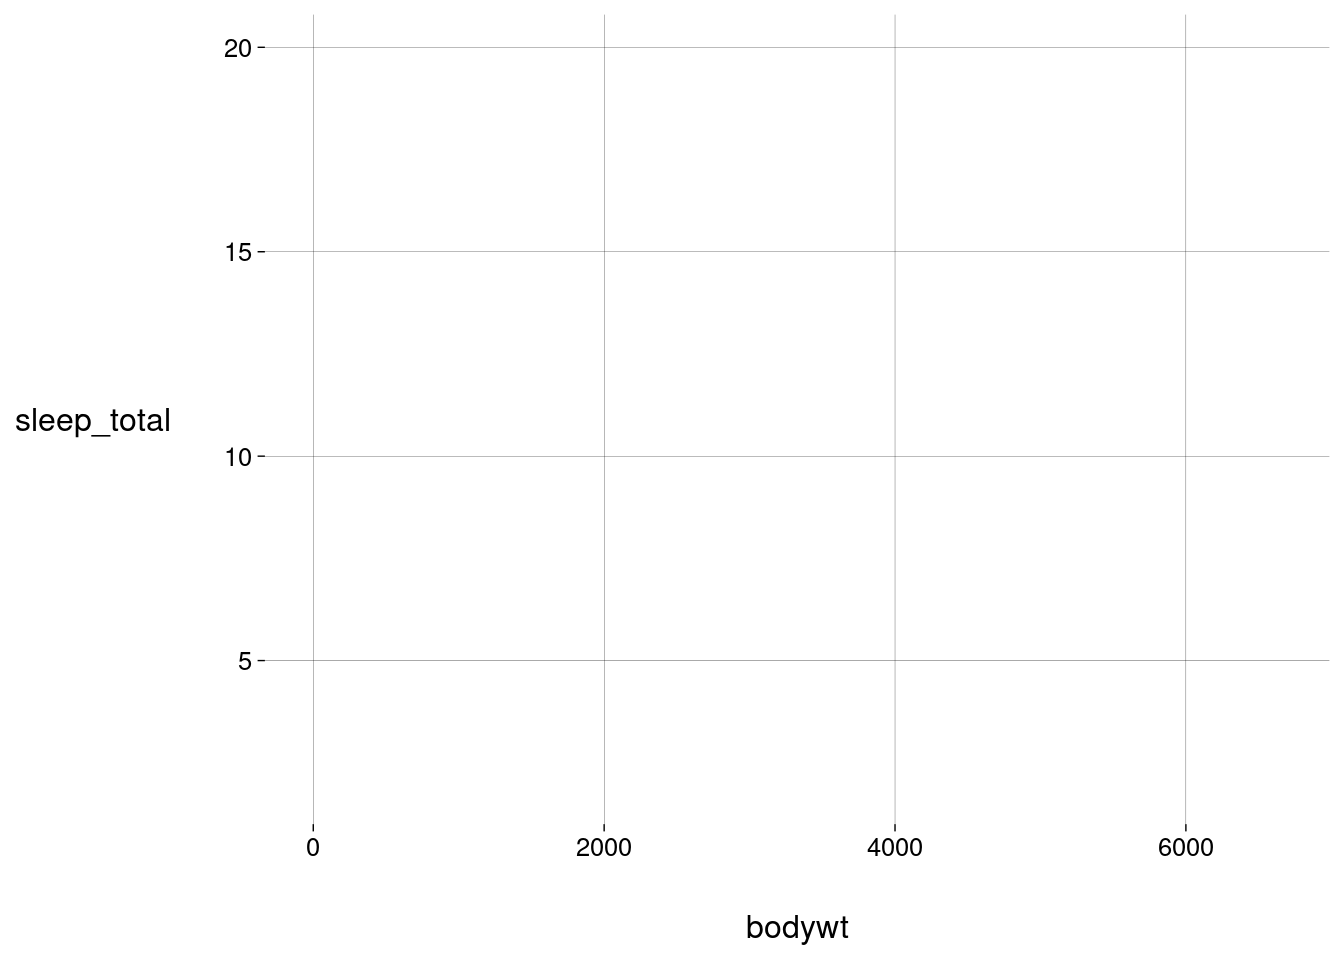
\includegraphics[width=1\linewidth]{_main_files/figure-latex/sono-peso-plot-1-1} \end{center}
\item
  O que houve? Cadê os pontos?
\item
  O problema foi que só especificamos o mapeamento estético (com \texttt{aes}, que são as iniciais de \emph{aesthetics}). {\hl{Faltou a geometria.}}

\begin{Shaded}
\begin{Highlighting}[]
\NormalTok{sono }\SpecialCharTok{\%\textgreater{}\%} 
  \FunctionTok{ggplot}\NormalTok{(}\FunctionTok{aes}\NormalTok{(}\AttributeTok{x =}\NormalTok{ bodywt, }\AttributeTok{y =}\NormalTok{ sleep\_total)) }\SpecialCharTok{+}
  \FunctionTok{geom\_point}\NormalTok{()}
\end{Highlighting}
\end{Shaded}

  \begin{center}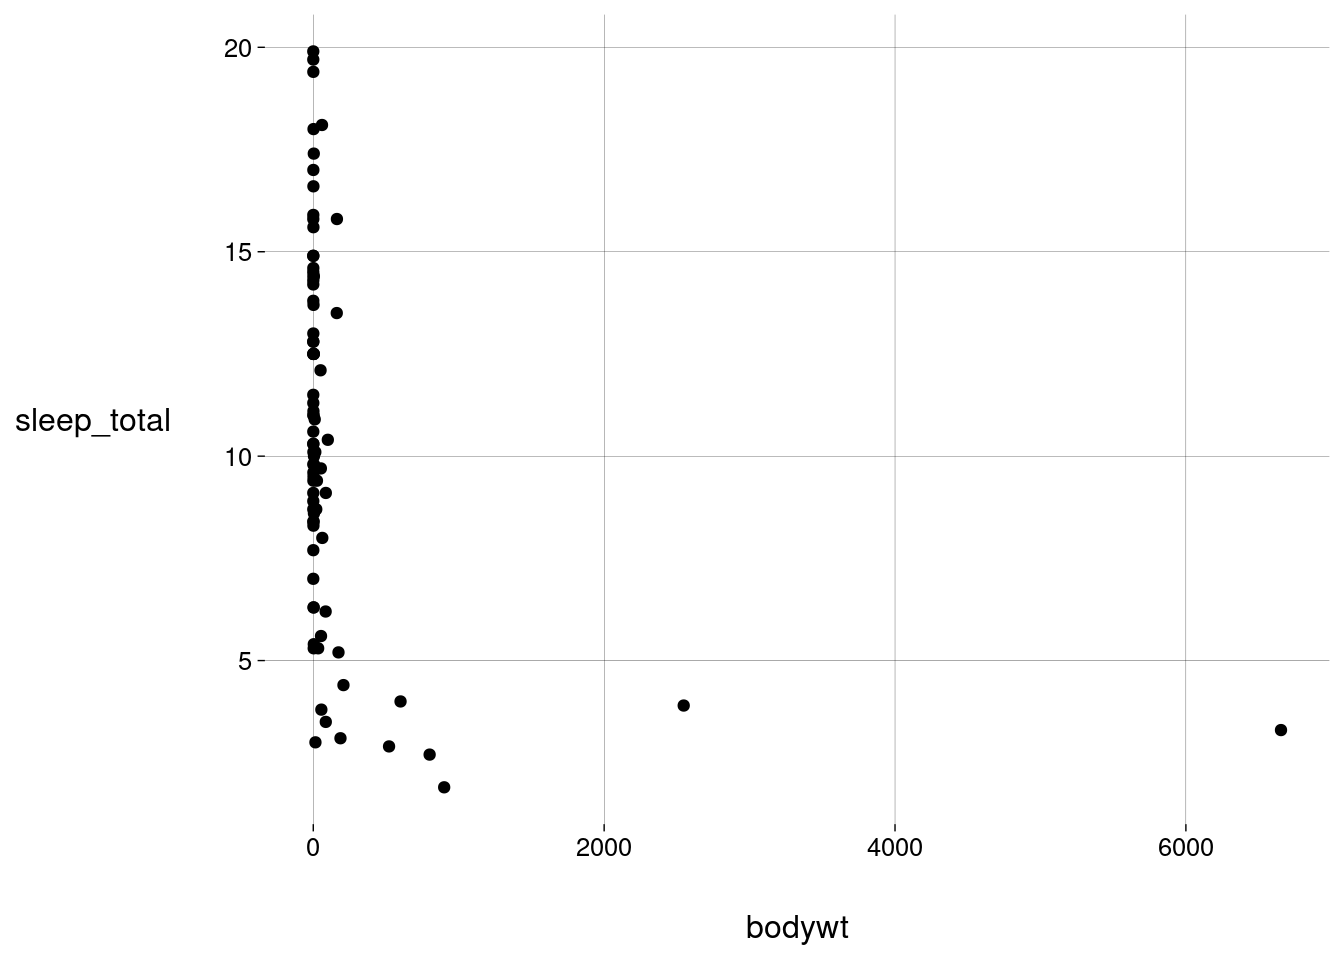
\includegraphics[width=1\linewidth]{_main_files/figure-latex/sono-peso-plot-2-1} \end{center}
\item
  Que horror.
\item
  A única coisa que percebemos aqui é que os mamíferos muito pesados dormem menos de \(5\) horas por noite.
\item
  Estes animais muito pesados estão estragando a escala do eixo \(x\).
\item
  Que animais são estes?

\begin{Shaded}
\begin{Highlighting}[]
\NormalTok{sono }\SpecialCharTok{\%\textgreater{}\%} 
  \FunctionTok{filter}\NormalTok{(bodywt }\SpecialCharTok{\textgreater{}} \DecValTok{250}\NormalTok{) }\SpecialCharTok{\%\textgreater{}\%} 
  \FunctionTok{select}\NormalTok{(name, bodywt) }\SpecialCharTok{\%\textgreater{}\%} 
  \FunctionTok{arrange}\NormalTok{(bodywt)}
\DocumentationTok{\#\# \# A tibble: 6 x 2}
\DocumentationTok{\#\#   name             bodywt}
\DocumentationTok{\#\#   \textless{}chr\textgreater{}             \textless{}dbl\textgreater{}}
\DocumentationTok{\#\# 1 Horse              521 }
\DocumentationTok{\#\# 2 Cow                600 }
\DocumentationTok{\#\# 3 Pilot whale        800 }
\DocumentationTok{\#\# 4 Giraffe            900.}
\DocumentationTok{\#\# 5 Asian elephant    2547 }
\DocumentationTok{\#\# 6 African elephant  6654}
\end{Highlighting}
\end{Shaded}
\item
  Além disso, há muitos pontos sobrepostos. Em bom português, temos um problema de \emph{overplotting}.
\item
  Existem diversas maneiras de lidar com isso.
\item
  A primeira delas é {\hl{alterando a opacidade dos pontos}}. Isto é um ajuste na geometria apenas, pois a opacidade, aqui, não representa informação nenhuma.

\begin{Shaded}
\begin{Highlighting}[]
\NormalTok{sono }\SpecialCharTok{\%\textgreater{}\%} 
  \FunctionTok{ggplot}\NormalTok{(}\FunctionTok{aes}\NormalTok{(}\AttributeTok{x =}\NormalTok{ bodywt, }\AttributeTok{y =}\NormalTok{ sleep\_total)) }\SpecialCharTok{+}
    \FunctionTok{geom\_point}\NormalTok{(}\AttributeTok{alpha =} \FloatTok{0.2}\NormalTok{)}
\end{Highlighting}
\end{Shaded}

  \begin{center}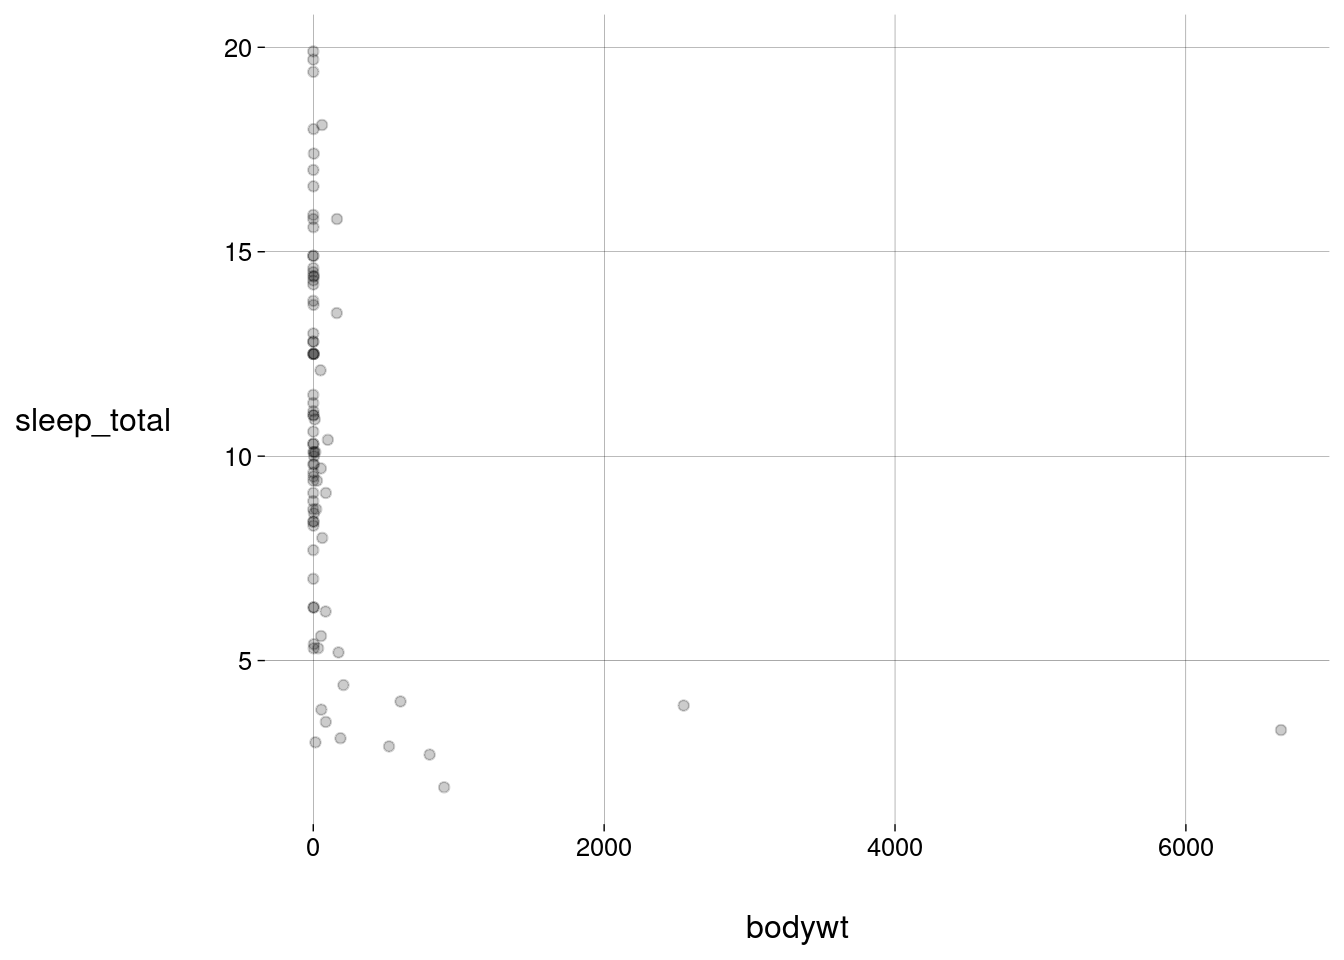
\includegraphics[width=1\linewidth]{_main_files/figure-latex/sono-peso-plot-alfa-1} \end{center}
\item
  Outra maneira é usar \texttt{geom\_jitter} em vez de \texttt{geom\_point}. ``\emph{Jitter}'' significa ``tremer''. As posições dos pontos são ligeiramente perturbadas, para evitar colisões. Perdemos precisão, mas a visualização fica melhor.

\begin{Shaded}
\begin{Highlighting}[]
\NormalTok{sono }\SpecialCharTok{\%\textgreater{}\%} 
  \FunctionTok{ggplot}\NormalTok{(}\FunctionTok{aes}\NormalTok{(}\AttributeTok{x =}\NormalTok{ bodywt, }\AttributeTok{y =}\NormalTok{ sleep\_total)) }\SpecialCharTok{+}
    \FunctionTok{geom\_jitter}\NormalTok{(}\AttributeTok{width =} \DecValTok{100}\NormalTok{)}
\end{Highlighting}
\end{Shaded}

  \begin{center}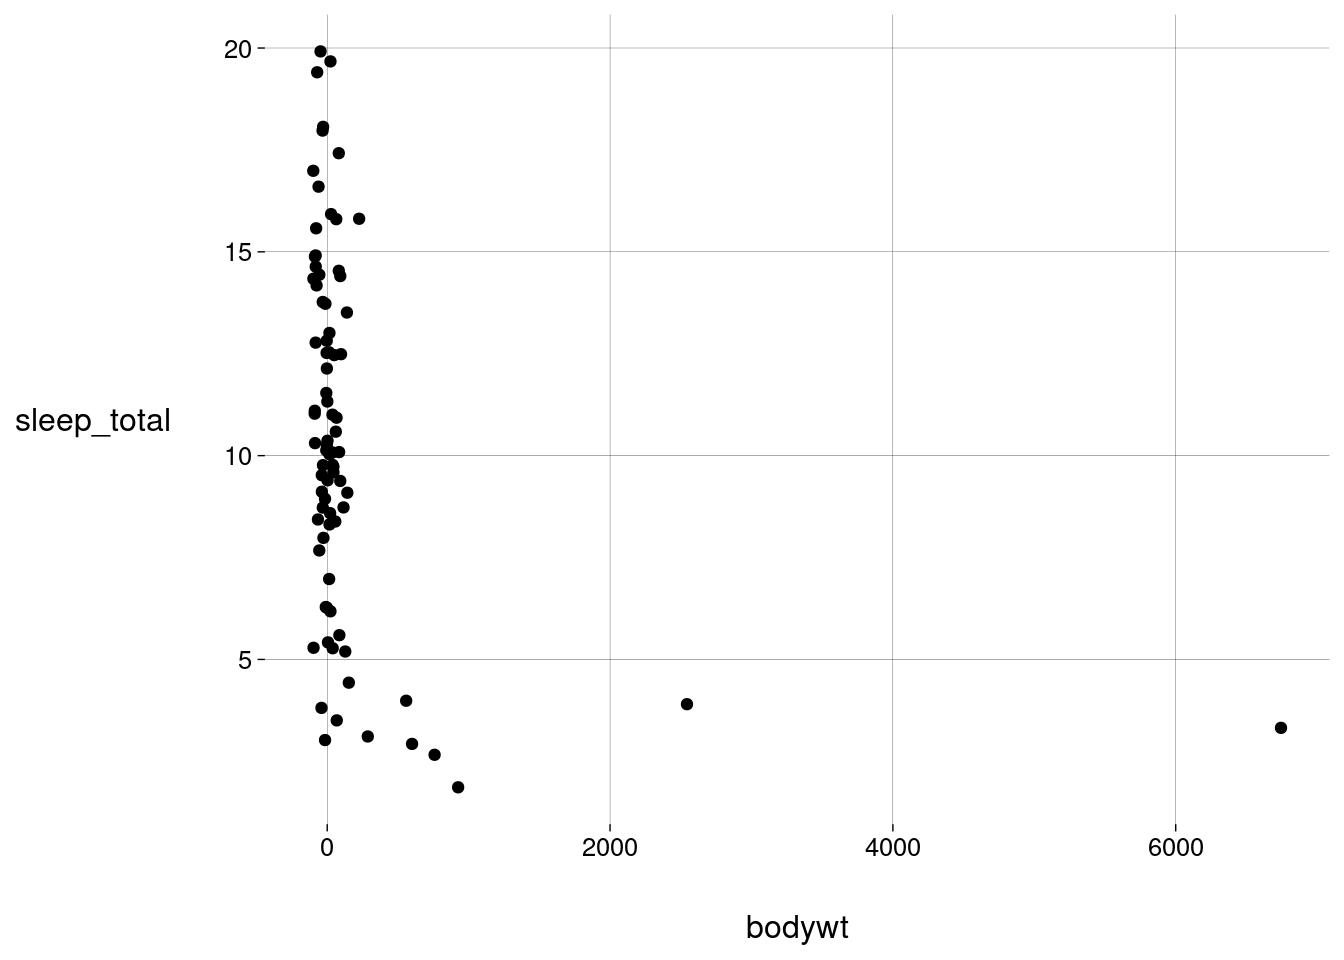
\includegraphics[width=1\linewidth]{_main_files/figure-latex/sono-peso-plot-jitter-1} \end{center}
\item
  Vamos mudar os limites do gráfico para nos concentrarmos nos animais menos pesados. Observe que {\hl{isto é um ajuste na escala}}.

\begin{Shaded}
\begin{Highlighting}[]
\NormalTok{sono }\SpecialCharTok{\%\textgreater{}\%} 
  \FunctionTok{ggplot}\NormalTok{(}\FunctionTok{aes}\NormalTok{(}\AttributeTok{x =}\NormalTok{ bodywt, }\AttributeTok{y =}\NormalTok{ sleep\_total)) }\SpecialCharTok{+}
    \FunctionTok{geom\_point}\NormalTok{() }\SpecialCharTok{+}
    \FunctionTok{scale\_x\_continuous}\NormalTok{(}\AttributeTok{limits =} \FunctionTok{c}\NormalTok{(}\DecValTok{0}\NormalTok{, }\DecValTok{200}\NormalTok{))}
\DocumentationTok{\#\# Warning: Removed 7 rows containing missing values (geom\_point).}
\end{Highlighting}
\end{Shaded}

  \begin{center}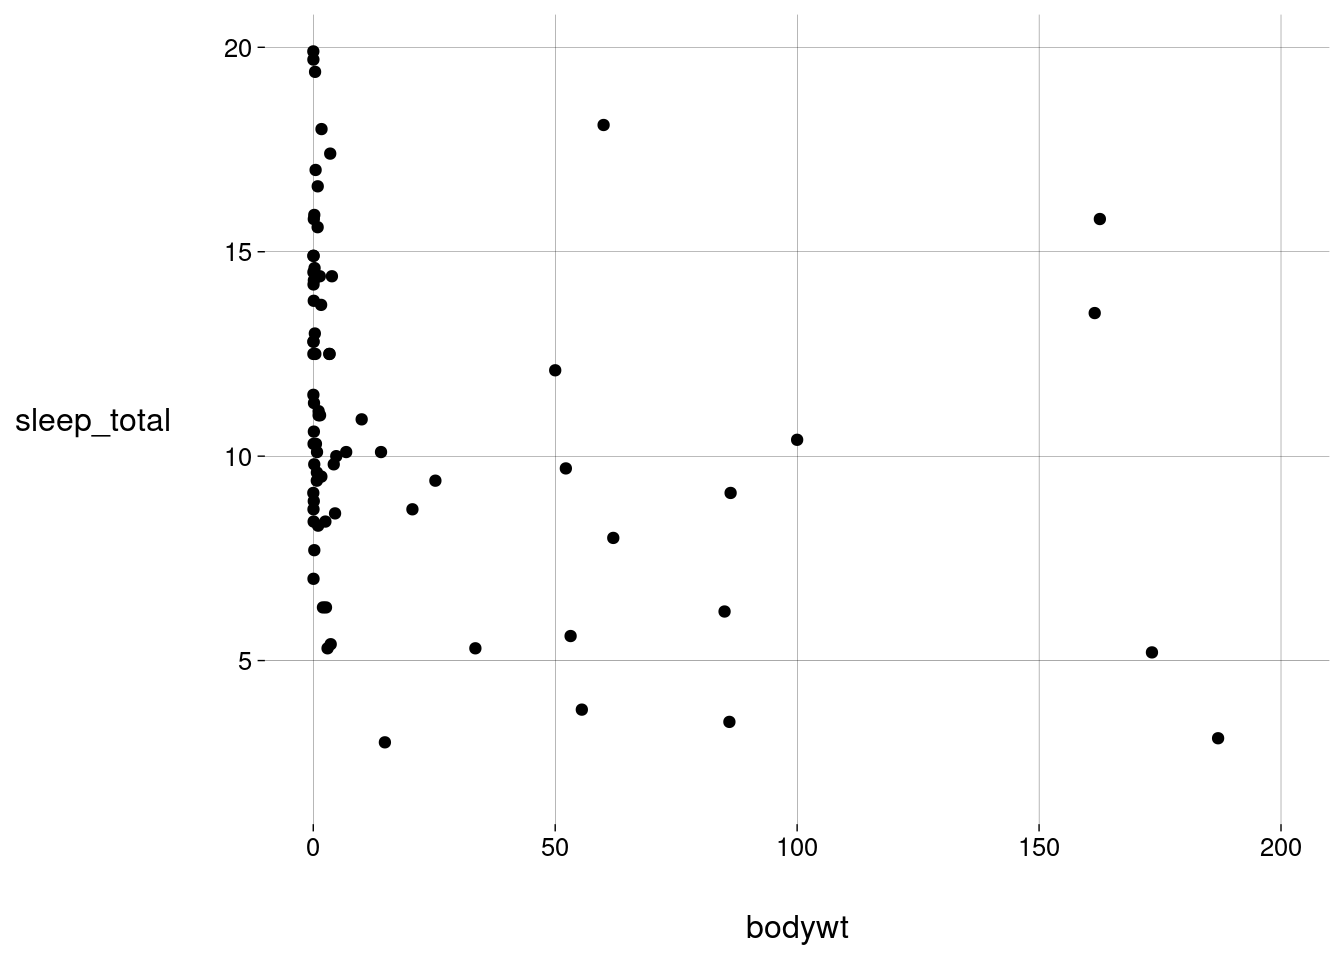
\includegraphics[width=1\linewidth]{_main_files/figure-latex/sono-peso-plot-3-1} \end{center}
\item
  Nestes limites, a relação entre horas de sono e peso não é mais tão pronunciada.
\end{itemize}

\hypertarget{horas-de-sono-e-peso-corporal-para-animais-pequenos}{%
\subsection{Horas de sono e peso corporal para animais pequenos}\label{horas-de-sono-e-peso-corporal-para-animais-pequenos}}

\begin{itemize}
\item
  Vamos restringir o gráfico a animais com no máximo \(5\)kg.

\begin{Shaded}
\begin{Highlighting}[]
\NormalTok{limite }\OtherTok{\textless{}{-}} \DecValTok{5}
\end{Highlighting}
\end{Shaded}
\item
  Em vez de mudar a escala do gráfico, vamos filtrar as linhas do \emph{data frame}:

\begin{Shaded}
\begin{Highlighting}[]
\NormalTok{sono }\SpecialCharTok{\%\textgreater{}\%} 
  \FunctionTok{filter}\NormalTok{(bodywt }\SpecialCharTok{\textless{}}\NormalTok{ limite) }\SpecialCharTok{\%\textgreater{}\%} 
  \FunctionTok{ggplot}\NormalTok{(}\FunctionTok{aes}\NormalTok{(}\AttributeTok{x =}\NormalTok{ bodywt, }\AttributeTok{y =}\NormalTok{ sleep\_total)) }\SpecialCharTok{+}
    \FunctionTok{geom\_point}\NormalTok{()}
\end{Highlighting}
\end{Shaded}

  \begin{center}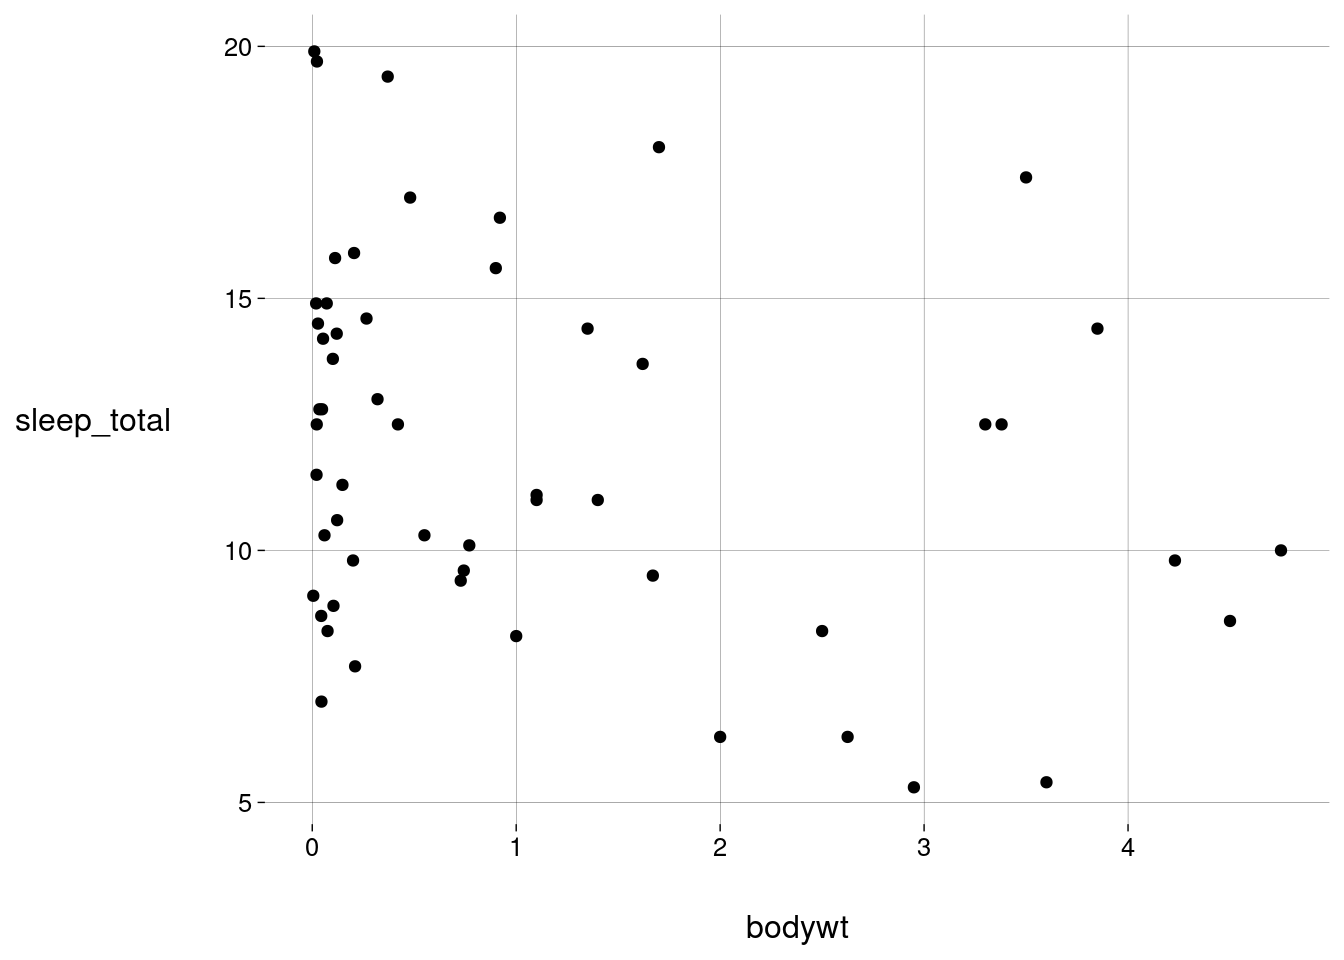
\includegraphics[width=1\linewidth]{_main_files/figure-latex/sono-peso-plot-pequenos-1} \end{center}
\end{itemize}

\hypertarget{incluindo-a-dieta}{%
\subsection{Incluindo a dieta}\label{incluindo-a-dieta}}

\begin{itemize}
\item
  Com a estética \texttt{color}. Observe como a legenda aparece automaticamente.

\begin{Shaded}
\begin{Highlighting}[]
\NormalTok{sono }\SpecialCharTok{\%\textgreater{}\%} 
  \FunctionTok{filter}\NormalTok{(bodywt }\SpecialCharTok{\textless{}}\NormalTok{ limite) }\SpecialCharTok{\%\textgreater{}\%} 
  \FunctionTok{ggplot}\NormalTok{(}\FunctionTok{aes}\NormalTok{(}\AttributeTok{x =}\NormalTok{ bodywt, }\AttributeTok{y =}\NormalTok{ sleep\_total, }\AttributeTok{color =}\NormalTok{ vore)) }\SpecialCharTok{+}
    \FunctionTok{geom\_point}\NormalTok{()}
\end{Highlighting}
\end{Shaded}

  \begin{center}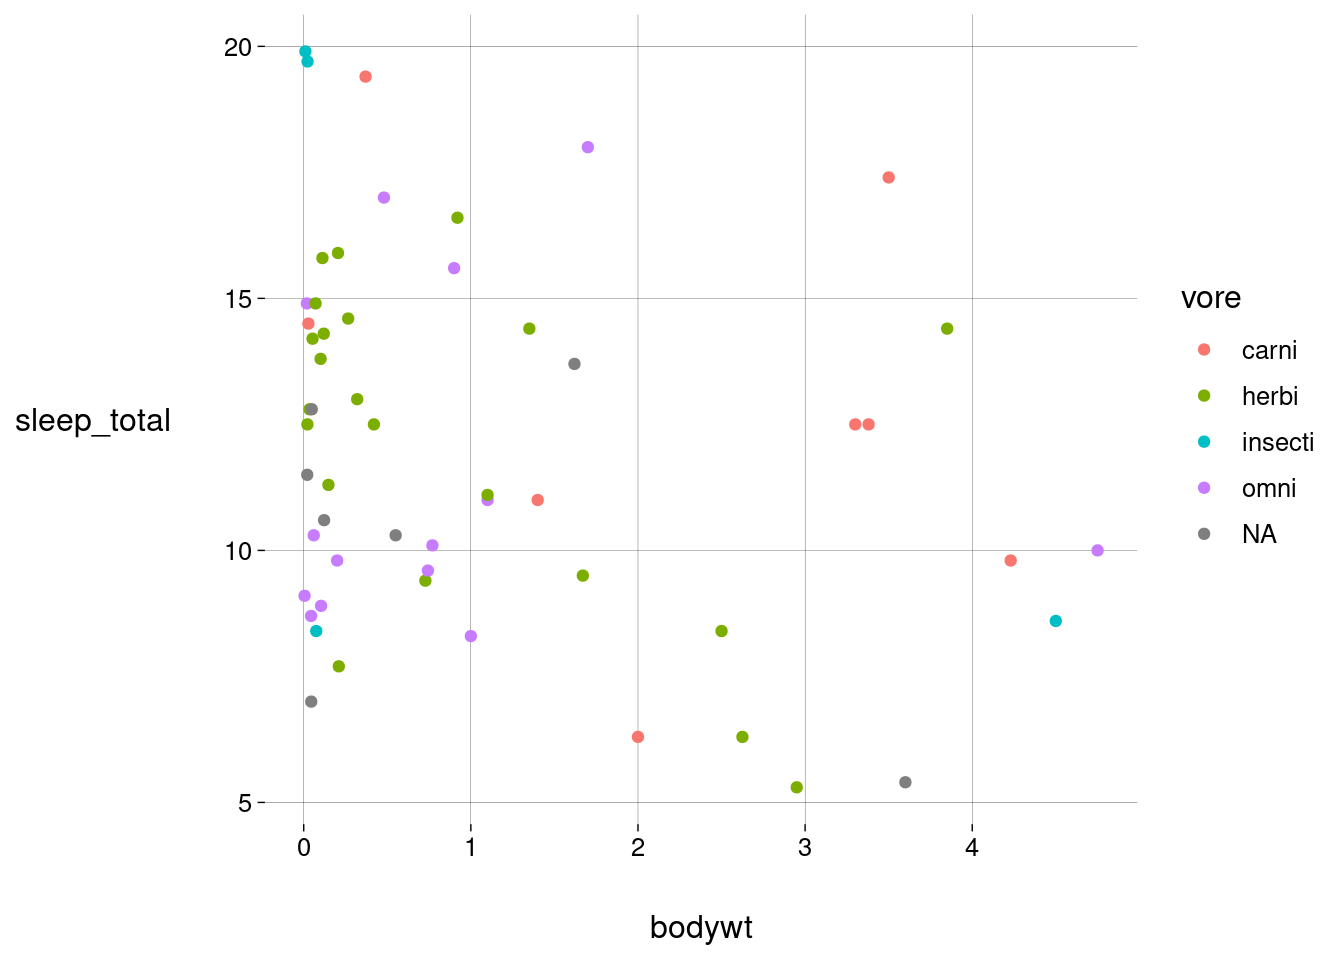
\includegraphics[width=1\linewidth]{_main_files/figure-latex/plot-sono-peso-dieta-1} \end{center}
\end{itemize}

\hypertarget{a-estuxe9tica-pode-ser-especificada-na-geom}{%
\subsection{\texorpdfstring{A estética pode ser especificada na \texttt{geom}}{A estética pode ser especificada na geom}}\label{a-estuxe9tica-pode-ser-especificada-na-geom}}

\begin{itemize}
\item
  Compare com o código anterior.

\begin{Shaded}
\begin{Highlighting}[]
\NormalTok{sono }\SpecialCharTok{\%\textgreater{}\%} 
  \FunctionTok{filter}\NormalTok{(bodywt }\SpecialCharTok{\textless{}}\NormalTok{ limite) }\SpecialCharTok{\%\textgreater{}\%} 
  \FunctionTok{ggplot}\NormalTok{() }\SpecialCharTok{+}
    \FunctionTok{geom\_point}\NormalTok{(}\FunctionTok{aes}\NormalTok{(}\AttributeTok{x =}\NormalTok{ bodywt, }\AttributeTok{y =}\NormalTok{ sleep\_total, }\AttributeTok{color =}\NormalTok{ vore))}
\end{Highlighting}
\end{Shaded}

  \begin{center}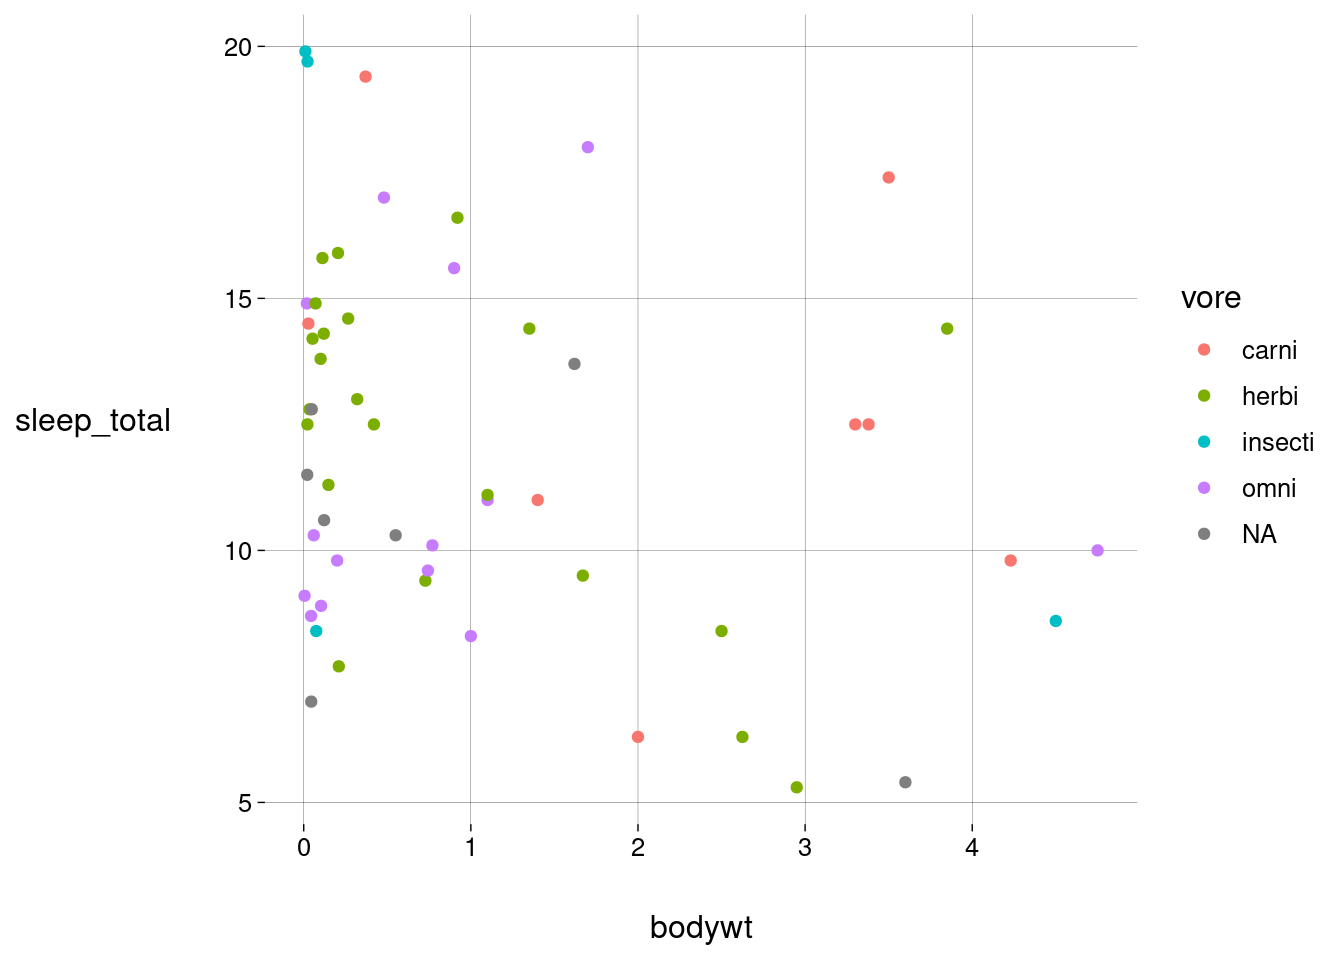
\includegraphics[width=1\linewidth]{_main_files/figure-latex/plot-sono-peso-dieta-geom-1} \end{center}
\item
  Fazendo deste modo, a estética só vale para uma geometria. Se você acrescentar outras geometrias (linhas, por exemplo), a estética não valerá para elas.
\end{itemize}

\hypertarget{aparuxeancia-fixa-ou-dependendo-de-variuxe1vel}{%
\subsection{Aparência fixa ou dependendo de variável?}\label{aparuxeancia-fixa-ou-dependendo-de-variuxe1vel}}

\begin{itemize}
\item
  Se for fixa, não é estética. Não representa informação.
\item
  Se depender de variável, é estética. Representa informação.
\item
  Compare o último \emph{chunk} acima com:

\begin{Shaded}
\begin{Highlighting}[]
\NormalTok{sono }\SpecialCharTok{\%\textgreater{}\%} 
  \FunctionTok{filter}\NormalTok{(bodywt }\SpecialCharTok{\textless{}}\NormalTok{ limite) }\SpecialCharTok{\%\textgreater{}\%} 
  \FunctionTok{ggplot}\NormalTok{() }\SpecialCharTok{+}
    \FunctionTok{geom\_point}\NormalTok{(}\FunctionTok{aes}\NormalTok{(}\AttributeTok{x =}\NormalTok{ bodywt, }\AttributeTok{y =}\NormalTok{ sleep\_total), }\AttributeTok{color =} \StringTok{\textquotesingle{}blue\textquotesingle{}}\NormalTok{)}
\end{Highlighting}
\end{Shaded}

  \begin{center}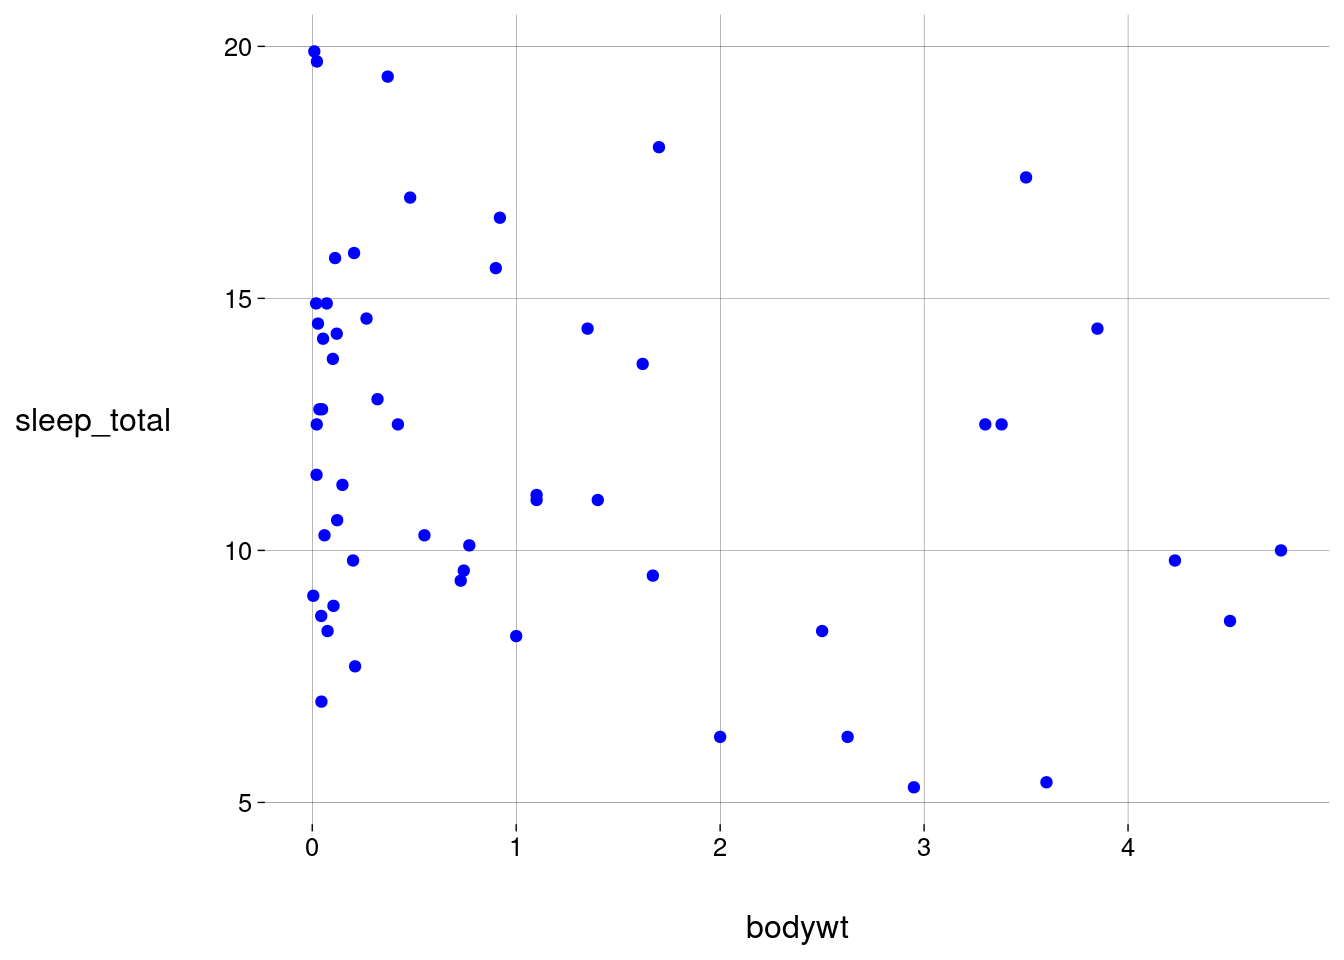
\includegraphics[width=1\linewidth]{_main_files/figure-latex/plot-sono-peso-cor-1} \end{center}
\item
  Se for uma estética, precisa estar {\hl{associada a uma variável}}, não a um valor fixo. Um erro comum seria fazer:

\begin{Shaded}
\begin{Highlighting}[]
\NormalTok{sono }\SpecialCharTok{\%\textgreater{}\%} 
  \FunctionTok{filter}\NormalTok{(bodywt }\SpecialCharTok{\textless{}}\NormalTok{ limite) }\SpecialCharTok{\%\textgreater{}\%} 
  \FunctionTok{ggplot}\NormalTok{() }\SpecialCharTok{+}
    \FunctionTok{geom\_point}\NormalTok{(}\FunctionTok{aes}\NormalTok{(}\AttributeTok{x =}\NormalTok{ bodywt, }\AttributeTok{y =}\NormalTok{ sleep\_total, }\AttributeTok{color =} \StringTok{\textquotesingle{}blue\textquotesingle{}}\NormalTok{))}
\end{Highlighting}
\end{Shaded}

  \begin{center}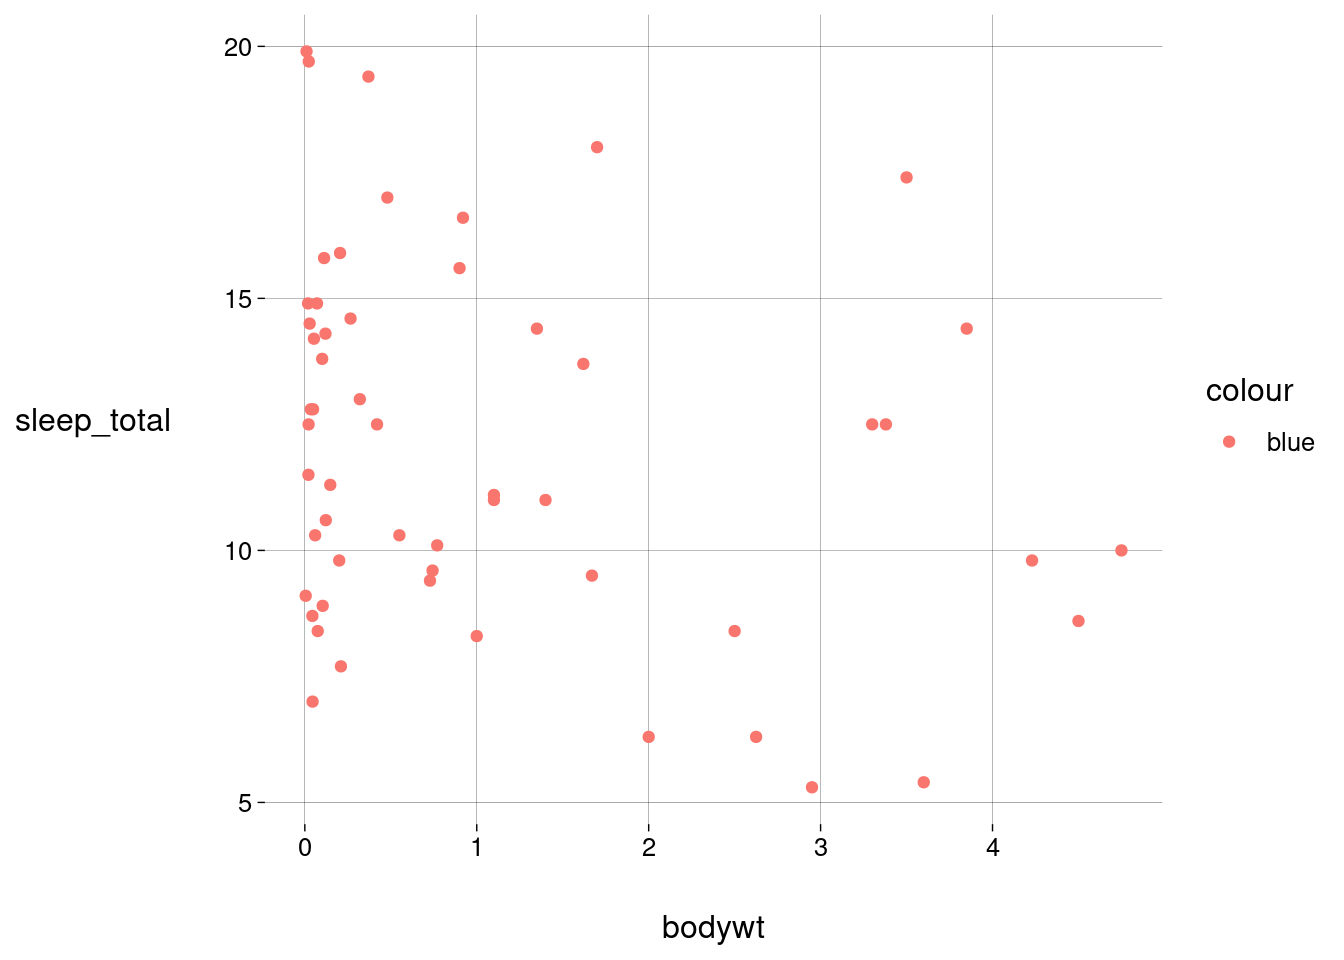
\includegraphics[width=1\linewidth]{_main_files/figure-latex/plot-sono-peso-cor-erro-1} \end{center}
\end{itemize}

\hypertarget{uma-correlauxe7uxe3o-mais-clara}{%
\subsection{Uma correlação mais clara}\label{uma-correlauxe7uxe3o-mais-clara}}

\begin{itemize}
\item
  Peso cerebral versus peso corporal:

\begin{Shaded}
\begin{Highlighting}[]
\NormalTok{sono }\SpecialCharTok{\%\textgreater{}\%} 
  \FunctionTok{ggplot}\NormalTok{() }\SpecialCharTok{+}
    \FunctionTok{geom\_point}\NormalTok{(}\FunctionTok{aes}\NormalTok{(}\AttributeTok{x =}\NormalTok{ bodywt, }\AttributeTok{y =}\NormalTok{ brainwt))}
\DocumentationTok{\#\# Warning: Removed 27 rows containing missing values (geom\_point).}
\end{Highlighting}
\end{Shaded}

  \begin{center}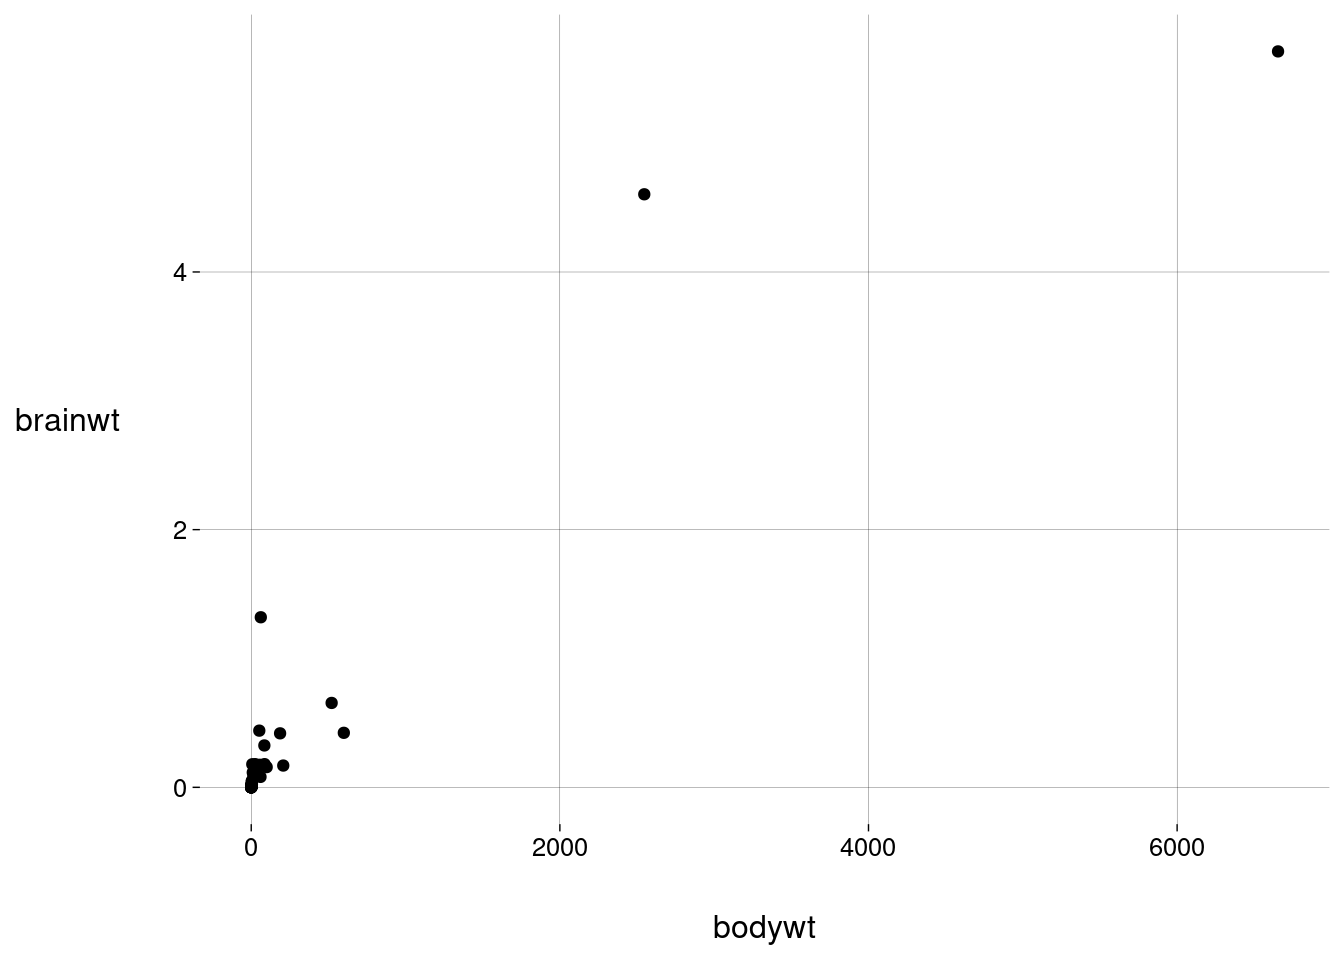
\includegraphics[width=1\linewidth]{_main_files/figure-latex/cerebro-corpo-1} \end{center}
\item
  Vamos restringir aos animais mais leves e mudar a opacidade:

\begin{Shaded}
\begin{Highlighting}[]
\NormalTok{sono }\SpecialCharTok{\%\textgreater{}\%} 
  \FunctionTok{filter}\NormalTok{(bodywt }\SpecialCharTok{\textless{}}\NormalTok{ limite) }\SpecialCharTok{\%\textgreater{}\%} 
  \FunctionTok{ggplot}\NormalTok{() }\SpecialCharTok{+}
    \FunctionTok{geom\_point}\NormalTok{(}\FunctionTok{aes}\NormalTok{(}\AttributeTok{x =}\NormalTok{ bodywt, }\AttributeTok{y =}\NormalTok{ brainwt), }\AttributeTok{alpha =}\NormalTok{ .}\DecValTok{5}\NormalTok{)}
\DocumentationTok{\#\# Warning: Removed 18 rows containing missing values (geom\_point).}
\end{Highlighting}
\end{Shaded}

  \begin{center}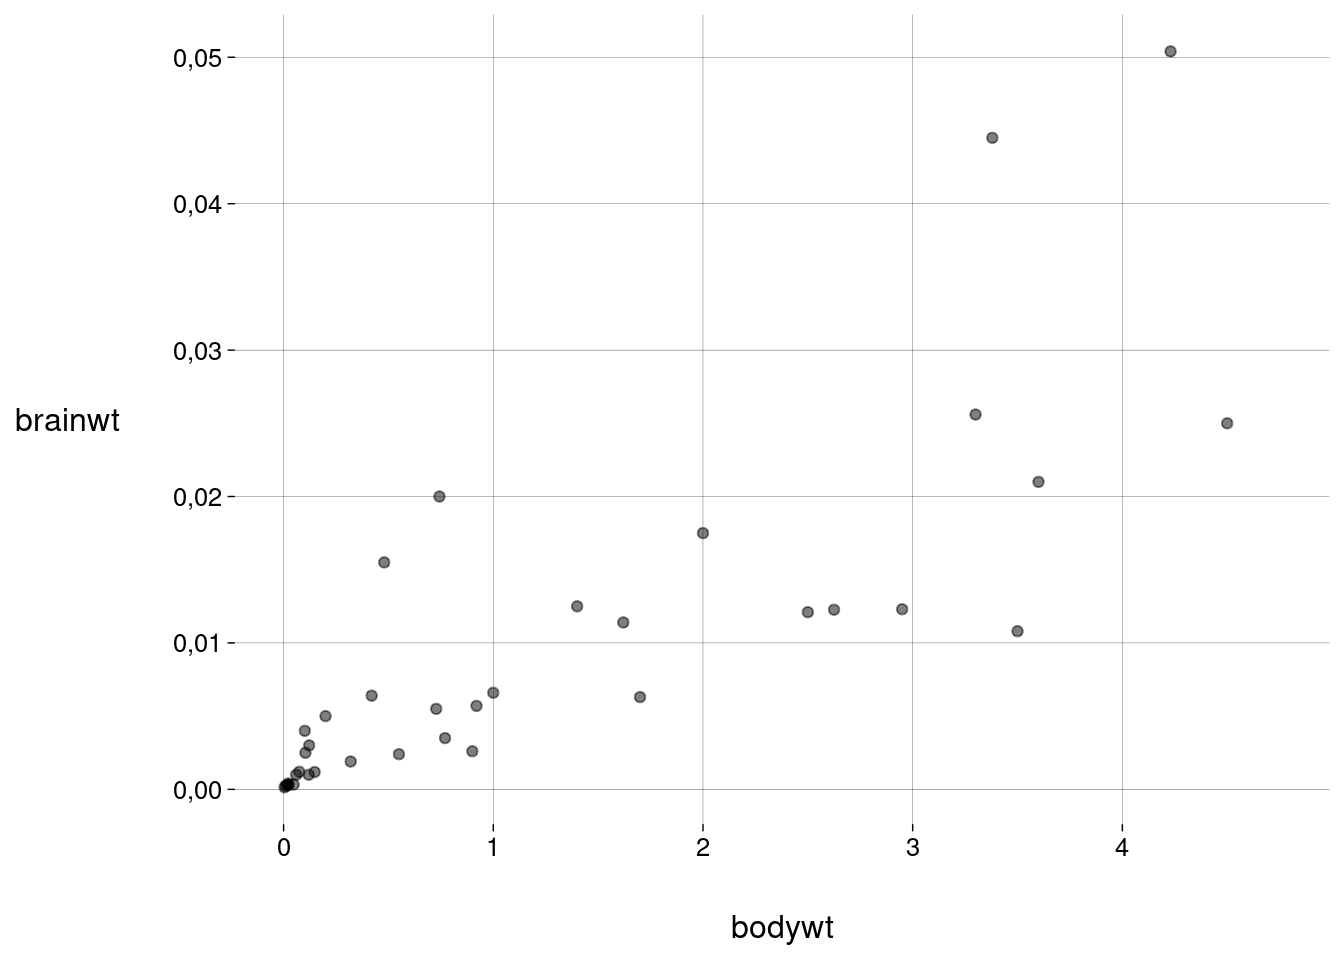
\includegraphics[width=1\linewidth]{_main_files/figure-latex/cerebro-corpo-2-1} \end{center}
\item
  Vamos incluir horas de sono e dieta. Observe as estéticas usadas.

\begin{Shaded}
\begin{Highlighting}[]
\NormalTok{sono }\SpecialCharTok{\%\textgreater{}\%} 
  \FunctionTok{filter}\NormalTok{(bodywt }\SpecialCharTok{\textless{}}\NormalTok{ limite) }\SpecialCharTok{\%\textgreater{}\%} 
  \FunctionTok{ggplot}\NormalTok{() }\SpecialCharTok{+}
    \FunctionTok{geom\_point}\NormalTok{(}
      \FunctionTok{aes}\NormalTok{(}
        \AttributeTok{x =}\NormalTok{ bodywt, }
        \AttributeTok{y =}\NormalTok{ brainwt,}
        \AttributeTok{size =}\NormalTok{ sleep\_total,}
        \AttributeTok{color =}\NormalTok{ vore}
\NormalTok{      ), }
      \AttributeTok{alpha =}\NormalTok{ .}\DecValTok{5}
\NormalTok{    )}
\DocumentationTok{\#\# Warning: Removed 18 rows containing missing values (geom\_point).}
\end{Highlighting}
\end{Shaded}

  \begin{center}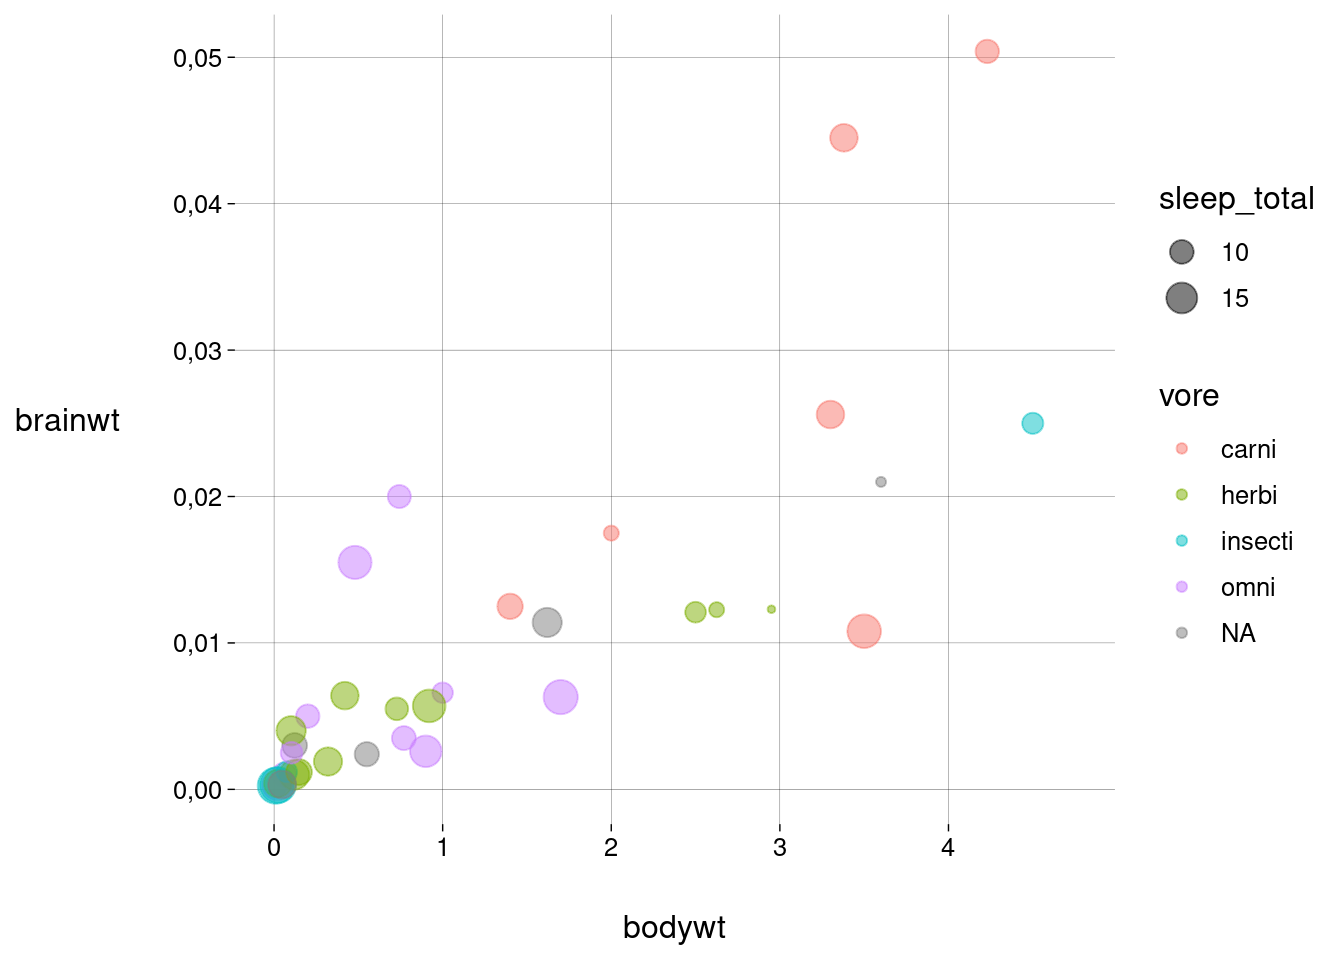
\includegraphics[width=1\linewidth]{_main_files/figure-latex/cerebro-corpo-3-1} \end{center}
\item
  Vamos mudar a escala dos tamanhos e incluir rótulos:

\begin{Shaded}
\begin{Highlighting}[]
\NormalTok{sono }\SpecialCharTok{\%\textgreater{}\%} 
  \FunctionTok{filter}\NormalTok{(bodywt }\SpecialCharTok{\textless{}}\NormalTok{ limite) }\SpecialCharTok{\%\textgreater{}\%} 
  \FunctionTok{ggplot}\NormalTok{() }\SpecialCharTok{+}
    \FunctionTok{geom\_point}\NormalTok{(}
      \FunctionTok{aes}\NormalTok{(}
        \AttributeTok{x =}\NormalTok{ bodywt, }
        \AttributeTok{y =}\NormalTok{ brainwt,}
        \AttributeTok{size =}\NormalTok{ sleep\_total,}
        \AttributeTok{color =}\NormalTok{ vore}
\NormalTok{      ), }
      \AttributeTok{alpha =}\NormalTok{ .}\DecValTok{5}
\NormalTok{    ) }\SpecialCharTok{+}
    \FunctionTok{scale\_size}\NormalTok{(}
      \AttributeTok{breaks =} \FunctionTok{seq}\NormalTok{(}\DecValTok{0}\NormalTok{, }\DecValTok{24}\NormalTok{, }\DecValTok{4}\NormalTok{)}
\NormalTok{    ) }\SpecialCharTok{+}
    \FunctionTok{labs}\NormalTok{(}
      \AttributeTok{title =} \StringTok{\textquotesingle{}Peso do cérebro versus peso corporal\textquotesingle{}}\NormalTok{,}
      \AttributeTok{subtitle =} \FunctionTok{paste0}\NormalTok{(}
        \StringTok{\textquotesingle{}para mamíferos com menos de \textquotesingle{}}\NormalTok{, }
\NormalTok{        limite, }
        \StringTok{\textquotesingle{} kg\textquotesingle{}}
\NormalTok{      ),}
      \AttributeTok{caption =} \StringTok{\textquotesingle{}Fonte: dataset \textasciigrave{}msleep\textasciigrave{}\textquotesingle{}}\NormalTok{,}
      \AttributeTok{x =} \StringTok{\textquotesingle{}Peso corporal (kg)\textquotesingle{}}\NormalTok{,}
      \AttributeTok{y =} \StringTok{\textquotesingle{}Peso do}\SpecialCharTok{\textbackslash{}n}\StringTok{ cérebro (kg)\textquotesingle{}}\NormalTok{,}
      \AttributeTok{color =} \StringTok{\textquotesingle{}Dieta\textquotesingle{}}\NormalTok{,}
      \AttributeTok{size =} \StringTok{\textquotesingle{}Horas}\SpecialCharTok{\textbackslash{}n}\StringTok{de sono\textquotesingle{}}
\NormalTok{    )}
\DocumentationTok{\#\# Warning: Removed 18 rows containing missing values (geom\_point).}
\end{Highlighting}
\end{Shaded}

  \begin{center}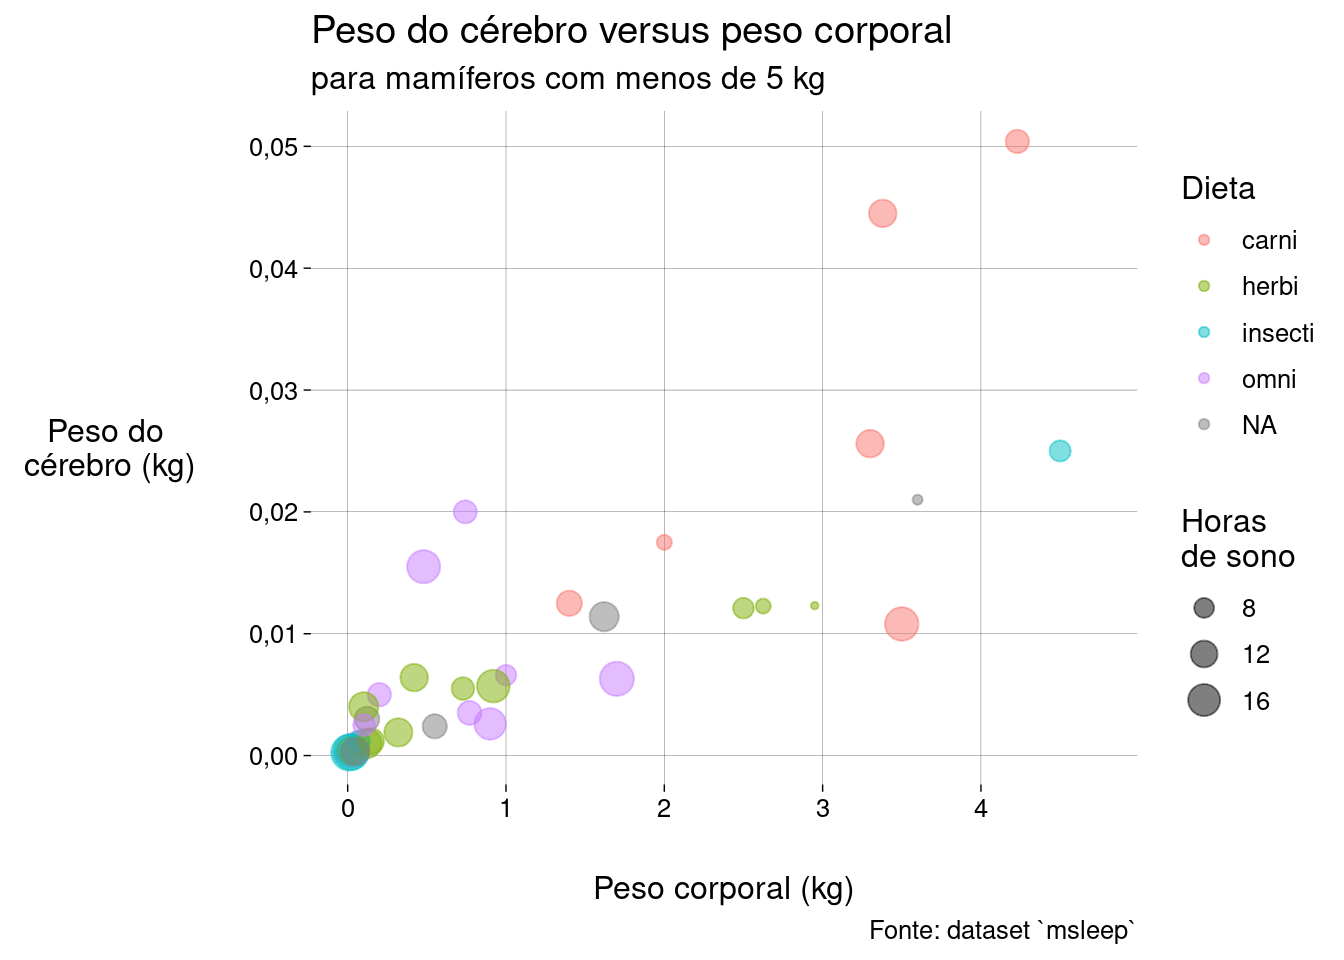
\includegraphics[width=1\linewidth]{_main_files/figure-latex/cerebro-corpo-4-1} \end{center}
\end{itemize}

\hypertarget{histogramas-e-cia.}{%
\section{Histogramas e cia.}\label{histogramas-e-cia.}}

\begin{itemize}
\tightlist
\item
  A idéia agora é {\hl{agrupar indivíduos em classes,}} dependendo do valor de uma variável quantitativa.
\end{itemize}

\hypertarget{distribuiuxe7uxf5es-de-frequuxeancia}{%
\subsection{Distribuições de frequência}\label{distribuiuxe7uxf5es-de-frequuxeancia}}

\begin{itemize}
\item
  Vamos nos concentrar nas horas de sono.

\begin{Shaded}
\begin{Highlighting}[]
\NormalTok{sono}\SpecialCharTok{$}\NormalTok{sleep\_total}
\DocumentationTok{\#\#  [1] 12,1 17,0 14,4 14,9  4,0 14,4  8,7  7,0 10,1  3,0  5,3  9,4 10,0}
\DocumentationTok{\#\# [14] 12,5 10,3  8,3  9,1 17,4  5,3 18,0  3,9 19,7  2,9  3,1 10,1 10,9}
\DocumentationTok{\#\# [27] 14,9 12,5  9,8  1,9  2,7  6,2  6,3  8,0  9,5  3,3 19,4 10,1 14,2}
\DocumentationTok{\#\# [40] 14,3 12,8 12,5 19,9 14,6 11,0  7,7 14,5  8,4  3,8  9,7 15,8 10,4}
\DocumentationTok{\#\# [53] 13,5  9,4 10,3 11,0 11,5 13,7  3,5  5,6 11,1 18,1  5,4 13,0  8,7}
\DocumentationTok{\#\# [66]  9,6  8,4 11,3 10,6 16,6 13,8 15,9 12,8  9,1  8,6 15,8  4,4 15,6}
\DocumentationTok{\#\# [79]  8,9  5,2  6,3 12,5  9,8}
\end{Highlighting}
\end{Shaded}
\item
  Antes de montar o histograma, vamos construir uma {\hl{distribuição de frequência.}}
\item
  A {\hl{amplitude}} é a diferença entre o valor máximo e o valor mínimo. A função \texttt{range} não retorna a amplitude, mas sim os valores mínimo e máximo:

\begin{Shaded}
\begin{Highlighting}[]
\NormalTok{sono}\SpecialCharTok{$}\NormalTok{sleep\_total }\SpecialCharTok{\%\textgreater{}\%} \FunctionTok{range}\NormalTok{()}
\DocumentationTok{\#\# [1]  1,9 19,9}
\end{Highlighting}
\end{Shaded}
\item
  Vamos decidir que cada classe vai ter \(2\) horas. A função \texttt{cut} substitui os valores do vetor pelos nomes das classes:

\begin{Shaded}
\begin{Highlighting}[]
\NormalTok{sono}\SpecialCharTok{$}\NormalTok{sleep\_total }\SpecialCharTok{\%\textgreater{}\%} 
  \FunctionTok{cut}\NormalTok{(}\AttributeTok{breaks =} \FunctionTok{seq}\NormalTok{(}\DecValTok{0}\NormalTok{, }\DecValTok{20}\NormalTok{, }\DecValTok{2}\NormalTok{), }\AttributeTok{right =} \ConstantTok{FALSE}\NormalTok{)}
\DocumentationTok{\#\#  [1] [12,14) [16,18) [14,16) [14,16) [4,6)   [14,16) [8,10)  [6,8)  }
\DocumentationTok{\#\#  [9] [10,12) [2,4)   [4,6)   [8,10)  [10,12) [12,14) [10,12) [8,10) }
\DocumentationTok{\#\# [17] [8,10)  [16,18) [4,6)   [18,20) [2,4)   [18,20) [2,4)   [2,4)  }
\DocumentationTok{\#\# [25] [10,12) [10,12) [14,16) [12,14) [8,10)  [0,2)   [2,4)   [6,8)  }
\DocumentationTok{\#\# [33] [6,8)   [8,10)  [8,10)  [2,4)   [18,20) [10,12) [14,16) [14,16)}
\DocumentationTok{\#\# [41] [12,14) [12,14) [18,20) [14,16) [10,12) [6,8)   [14,16) [8,10) }
\DocumentationTok{\#\# [49] [2,4)   [8,10)  [14,16) [10,12) [12,14) [8,10)  [10,12) [10,12)}
\DocumentationTok{\#\# [57] [10,12) [12,14) [2,4)   [4,6)   [10,12) [18,20) [4,6)   [12,14)}
\DocumentationTok{\#\# [65] [8,10)  [8,10)  [8,10)  [10,12) [10,12) [16,18) [12,14) [14,16)}
\DocumentationTok{\#\# [73] [12,14) [8,10)  [8,10)  [14,16) [4,6)   [14,16) [8,10)  [4,6)  }
\DocumentationTok{\#\# [81] [6,8)   [12,14) [8,10) }
\DocumentationTok{\#\# 10 Levels: [0,2) [2,4) [4,6) [6,8) [8,10) [10,12) [12,14) ... [18,20)}
\end{Highlighting}
\end{Shaded}
\item
  A função \texttt{table} faz a contagem dos elementos de cada classe:

\begin{Shaded}
\begin{Highlighting}[]
\NormalTok{sono}\SpecialCharTok{$}\NormalTok{sleep\_total }\SpecialCharTok{\%\textgreater{}\%}  
  \FunctionTok{cut}\NormalTok{(}\AttributeTok{breaks =} \FunctionTok{seq}\NormalTok{(}\DecValTok{0}\NormalTok{, }\DecValTok{20}\NormalTok{, }\DecValTok{2}\NormalTok{), }\AttributeTok{right =} \ConstantTok{FALSE}\NormalTok{) }\SpecialCharTok{\%\textgreater{}\%} 
  \FunctionTok{table}\NormalTok{(}\AttributeTok{dnn =} \StringTok{\textquotesingle{}Horas de sono\textquotesingle{}}\NormalTok{) }\SpecialCharTok{\%\textgreater{}\%} 
  \FunctionTok{as.data.frame}\NormalTok{()}
\DocumentationTok{\#\# \# A tibble: 10 x 2}
\DocumentationTok{\#\#   Horas.de.sono  Freq}
\DocumentationTok{\#\#   \textless{}fct\textgreater{}         \textless{}int\textgreater{}}
\DocumentationTok{\#\# 1 [0,2)             1}
\DocumentationTok{\#\# 2 [2,4)             8}
\DocumentationTok{\#\# 3 [4,6)             7}
\DocumentationTok{\#\# 4 [6,8)             5}
\DocumentationTok{\#\# 5 [8,10)           17}
\DocumentationTok{\#\# 6 [10,12)          14}
\DocumentationTok{\#\# \# ... with 4 more rows}
\end{Highlighting}
\end{Shaded}
\end{itemize}

\hypertarget{histograma}{%
\subsection{Histograma}\label{histograma}}

\begin{itemize}
\item
  Na verdade, o \texttt{ggplot2} já faz esses cálculos para nós.
\item
  O \emph{default} é criar \(30\) classes (\emph{bins}):

\begin{Shaded}
\begin{Highlighting}[]
\NormalTok{sono }\SpecialCharTok{\%\textgreater{}\%} 
  \FunctionTok{ggplot}\NormalTok{(}\FunctionTok{aes}\NormalTok{(}\AttributeTok{x =}\NormalTok{ sleep\_total)) }\SpecialCharTok{+}
    \FunctionTok{geom\_histogram}\NormalTok{()}
\DocumentationTok{\#\# \textasciigrave{}stat\_bin()\textasciigrave{} using \textasciigrave{}bins = 30\textasciigrave{}. Pick better value with \textasciigrave{}binwidth\textasciigrave{}.}
\end{Highlighting}
\end{Shaded}

  \begin{center}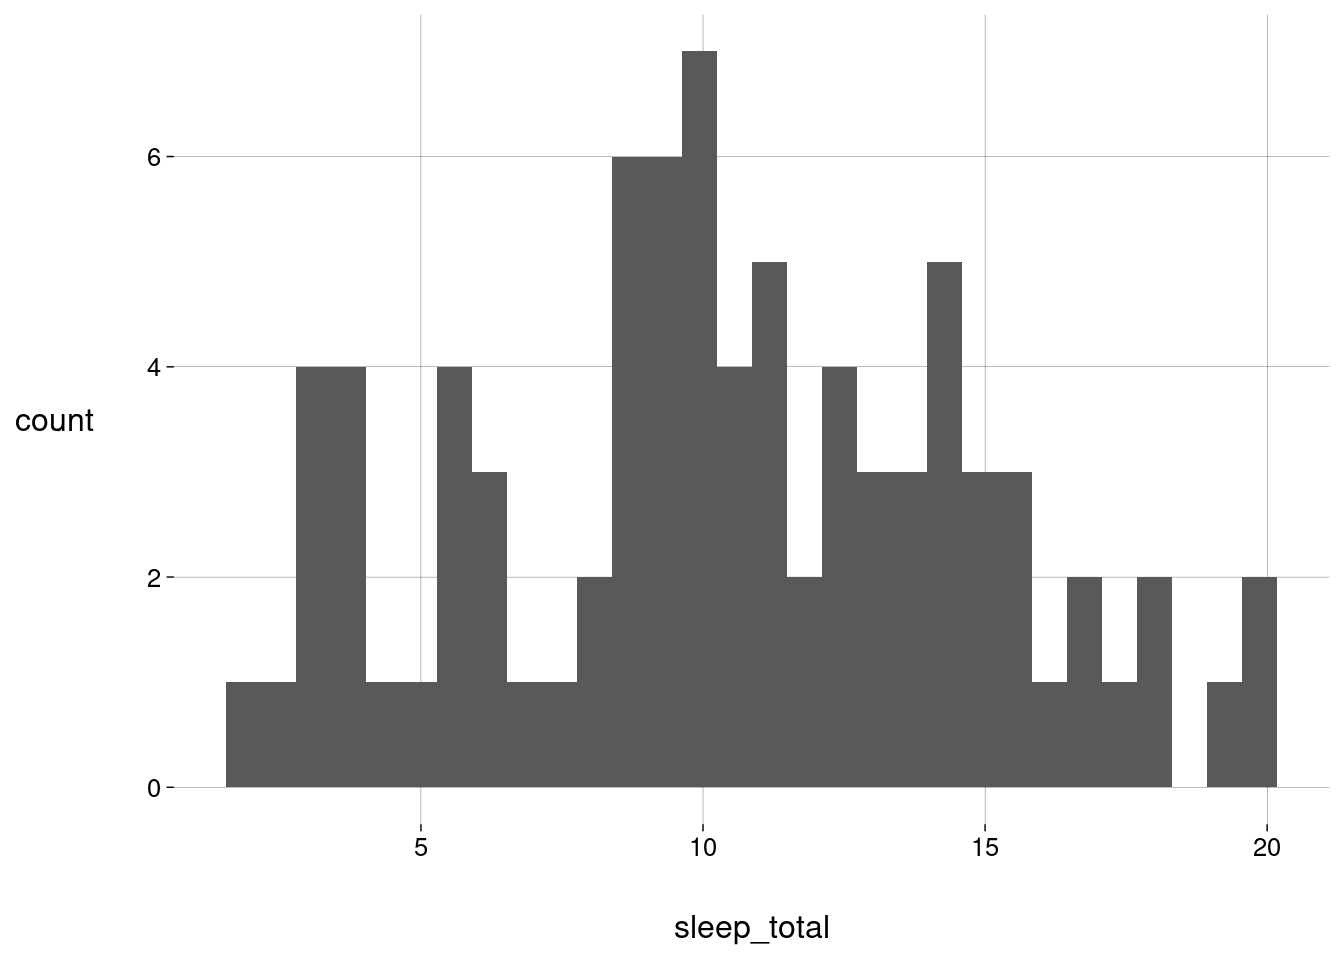
\includegraphics[width=1\linewidth]{_main_files/figure-latex/hist-sono1-1} \end{center}
\item
  Vamos mudar isto passando um vetor de limites das classes (\emph{breaks}):

\begin{Shaded}
\begin{Highlighting}[]
\NormalTok{sono }\SpecialCharTok{\%\textgreater{}\%} 
  \FunctionTok{ggplot}\NormalTok{(}\FunctionTok{aes}\NormalTok{(}\AttributeTok{x =}\NormalTok{ sleep\_total)) }\SpecialCharTok{+}
    \FunctionTok{geom\_histogram}\NormalTok{(}\AttributeTok{breaks =} \FunctionTok{seq}\NormalTok{(}\DecValTok{0}\NormalTok{, }\DecValTok{20}\NormalTok{, }\DecValTok{2}\NormalTok{)) }\SpecialCharTok{+}
    \FunctionTok{scale\_x\_continuous}\NormalTok{(}\AttributeTok{breaks =} \FunctionTok{seq}\NormalTok{(}\DecValTok{0}\NormalTok{, }\DecValTok{20}\NormalTok{, }\DecValTok{2}\NormalTok{))}
\end{Highlighting}
\end{Shaded}

  \begin{center}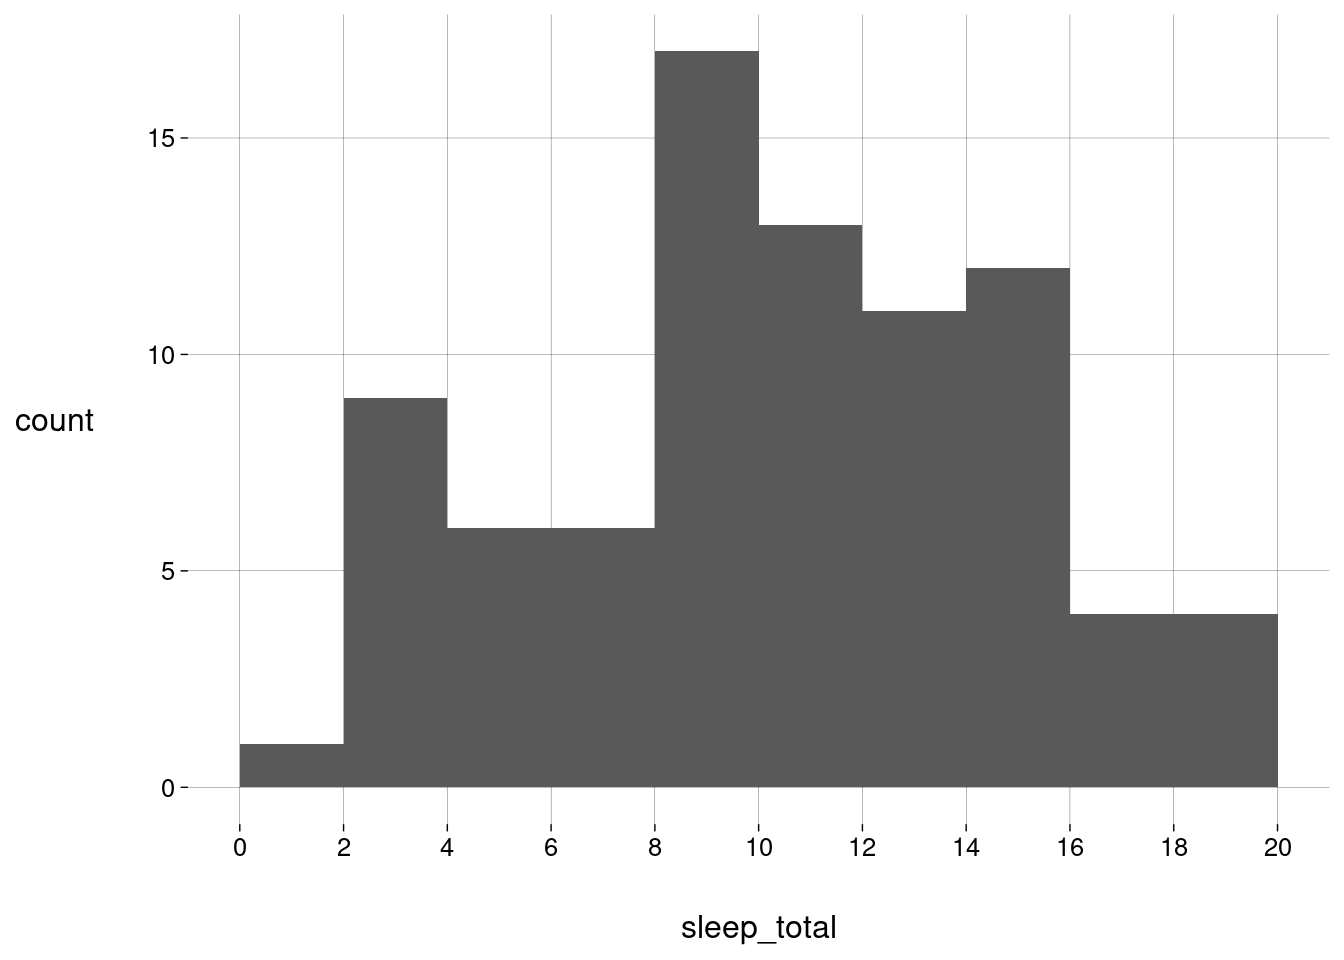
\includegraphics[width=1\linewidth]{_main_files/figure-latex/hist-sono2-1} \end{center}
\end{itemize}

\hypertarget{poluxedgono-de-frequuxeancia}{%
\subsection{Polígono de frequência}\label{poluxedgono-de-frequuxeancia}}

\begin{itemize}
\item
  Em vez das barras do histograma, podemos desenhar uma linha ligando seus topos.
\item
  O resultado é um {\hl{polígono de frequência}}.

\begin{Shaded}
\begin{Highlighting}[]
\NormalTok{pf }\OtherTok{\textless{}{-}}\NormalTok{ sono }\SpecialCharTok{\%\textgreater{}\%} 
  \FunctionTok{ggplot}\NormalTok{(}\FunctionTok{aes}\NormalTok{(}\AttributeTok{x =}\NormalTok{ sleep\_total)) }\SpecialCharTok{+}
    \FunctionTok{geom\_freqpoly}\NormalTok{(}\AttributeTok{breaks =} \FunctionTok{seq}\NormalTok{(}\DecValTok{0}\NormalTok{, }\DecValTok{20}\NormalTok{, }\DecValTok{2}\NormalTok{), }\AttributeTok{color =} \StringTok{\textquotesingle{}red\textquotesingle{}}\NormalTok{) }\SpecialCharTok{+}
    \FunctionTok{scale\_x\_continuous}\NormalTok{(}\AttributeTok{breaks =} \FunctionTok{seq}\NormalTok{(}\DecValTok{0}\NormalTok{, }\DecValTok{20}\NormalTok{, }\DecValTok{2}\NormalTok{))}

\NormalTok{pf}
\end{Highlighting}
\end{Shaded}

  \begin{center}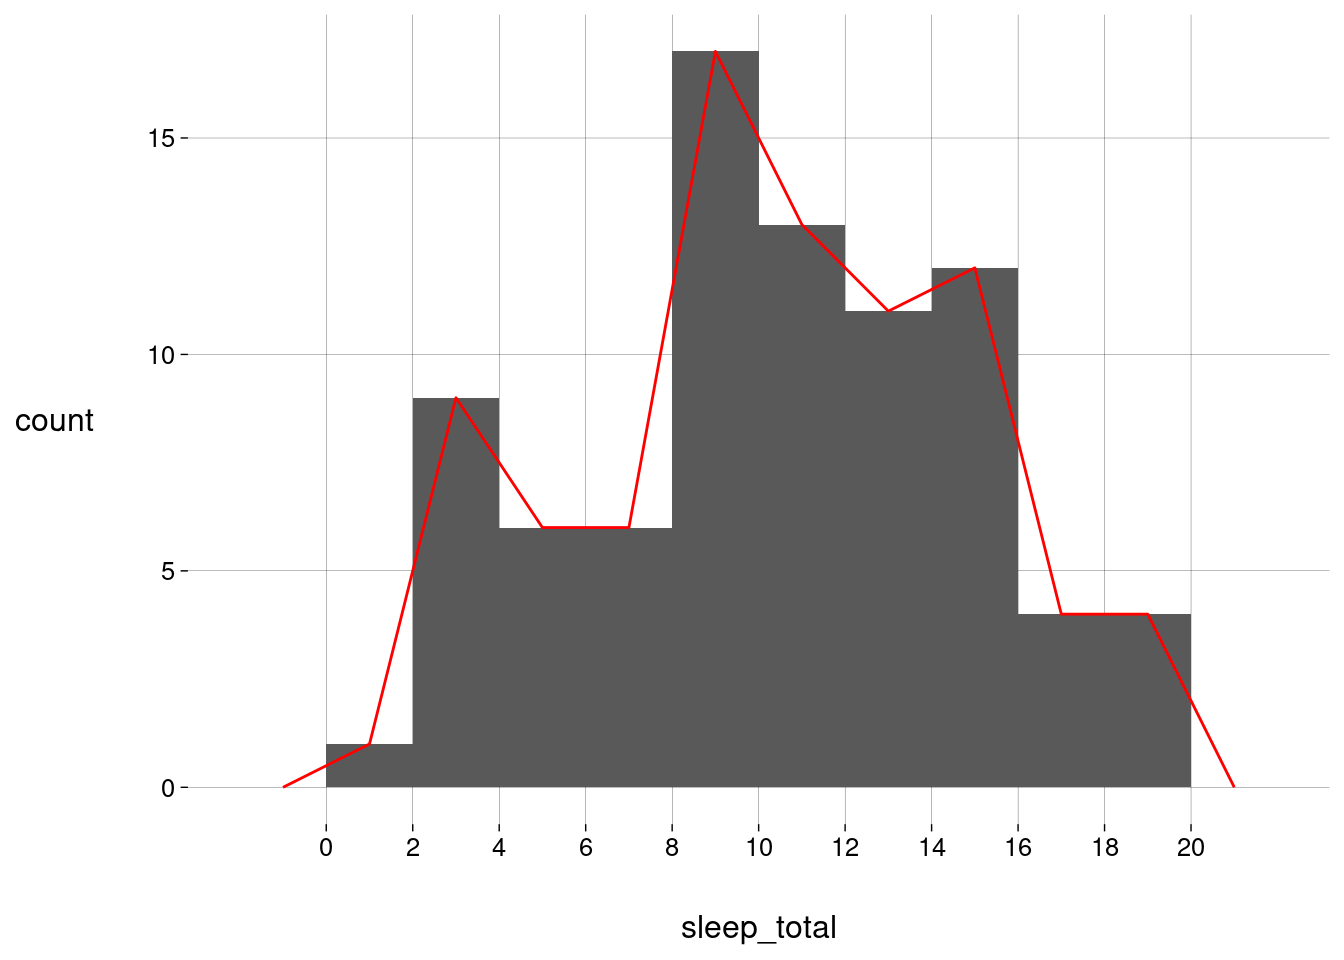
\includegraphics[width=1\linewidth]{_main_files/figure-latex/hist-freqpoly-1} \end{center}
\item
  Vamos sobrepor o polígono de frequência ao histograma, para deixar claro o que está acontecendo:

\begin{Shaded}
\begin{Highlighting}[]
\NormalTok{pf }\SpecialCharTok{+} \FunctionTok{geom\_histogram}\NormalTok{(}\AttributeTok{breaks =} \FunctionTok{seq}\NormalTok{(}\DecValTok{0}\NormalTok{, }\DecValTok{20}\NormalTok{, }\DecValTok{2}\NormalTok{), }\AttributeTok{alpha =}\NormalTok{ .}\DecValTok{3}\NormalTok{)}
\end{Highlighting}
\end{Shaded}

  \begin{center}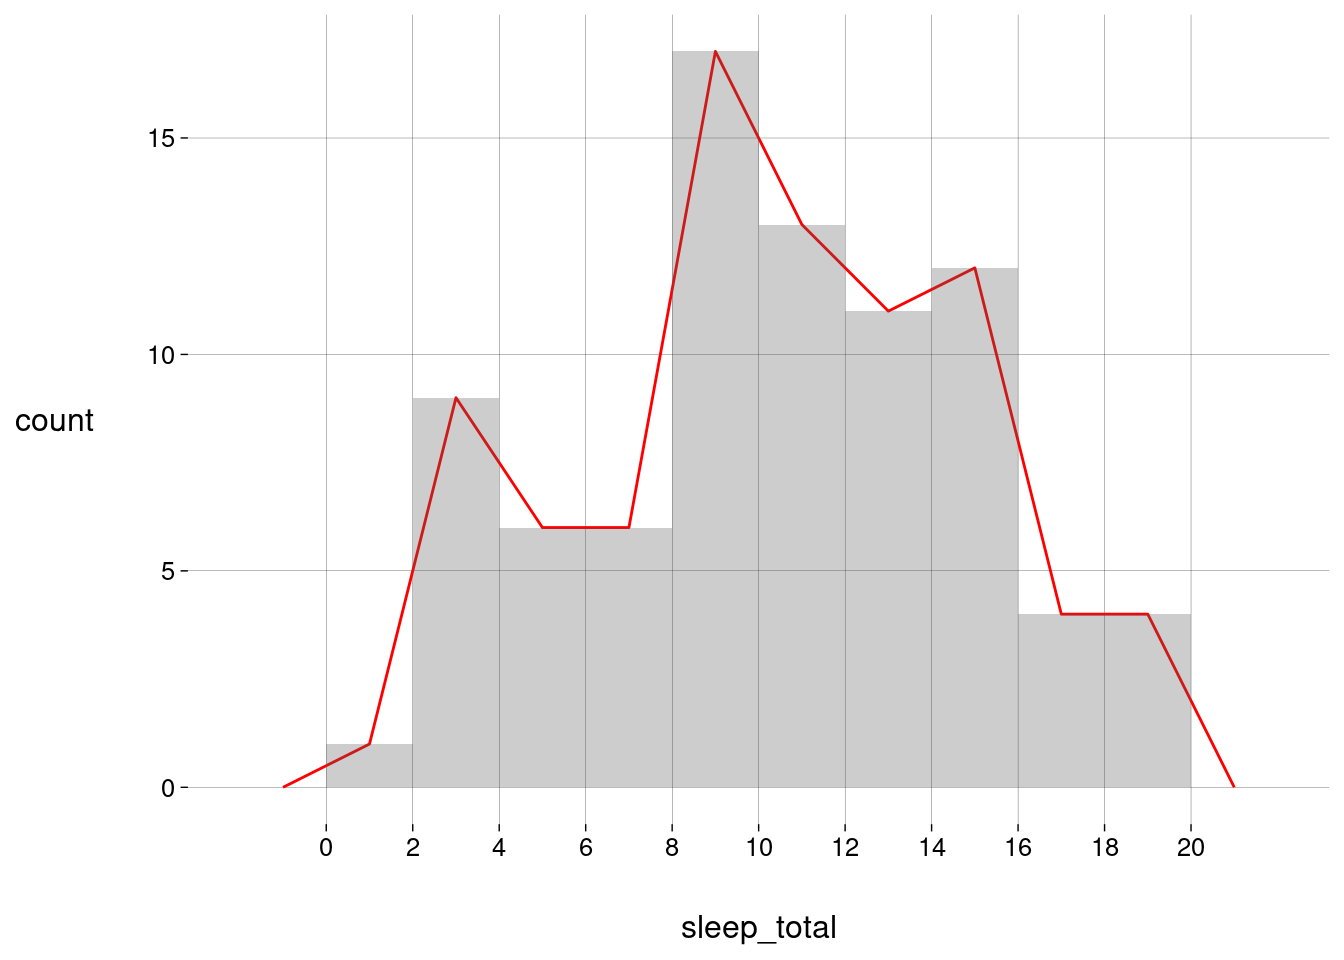
\includegraphics[width=1\linewidth]{_main_files/figure-latex/hist-freqpoly2-1} \end{center}
\end{itemize}

\hypertarget{ogiva}{%
\section{Ogiva}\label{ogiva}}

\begin{itemize}
\item
  A ogiva é um gráfico que mostra a {\hl{frequência acumulada}}: para cada valor \(v\) da variável no eixo \(x\), a proporção de indivíduos com valor menor ou igual a \(v\).
\item
  A geometria \texttt{geom\_step} gera o gráfico de uma {\hl{função degrau}}.
\item
  Cada geometria está ligada a uma {[}\texttt{stat}{]}, um algoritmo para computar o que vai ser desenhado. Aqui, passamos para a geometria {\hl{a função \texttt{ecdf} (\emph{empirical cumulative distribution function}), que calcula as frequências acumuladas.}}

\begin{Shaded}
\begin{Highlighting}[]
\NormalTok{sono }\SpecialCharTok{\%\textgreater{}\%} 
  \FunctionTok{ggplot}\NormalTok{(}\FunctionTok{aes}\NormalTok{(}\AttributeTok{x =}\NormalTok{ sleep\_total)) }\SpecialCharTok{+}
    \FunctionTok{geom\_step}\NormalTok{(}\AttributeTok{stat =} \StringTok{\textquotesingle{}ecdf\textquotesingle{}}\NormalTok{) }\SpecialCharTok{+}
    \FunctionTok{scale\_x\_continuous}\NormalTok{(}\AttributeTok{breaks =} \FunctionTok{seq}\NormalTok{(}\DecValTok{0}\NormalTok{, }\DecValTok{20}\NormalTok{, }\DecValTok{2}\NormalTok{)) }\SpecialCharTok{+}
    \FunctionTok{scale\_y\_continuous}\NormalTok{(}\AttributeTok{breaks =} \FunctionTok{seq}\NormalTok{(}\DecValTok{0}\NormalTok{, }\DecValTok{1}\NormalTok{, .}\DecValTok{1}\NormalTok{)) }\SpecialCharTok{+}
    \FunctionTok{labs}\NormalTok{(}\AttributeTok{y =} \ConstantTok{NULL}\NormalTok{)}
\end{Highlighting}
\end{Shaded}

  \begin{center}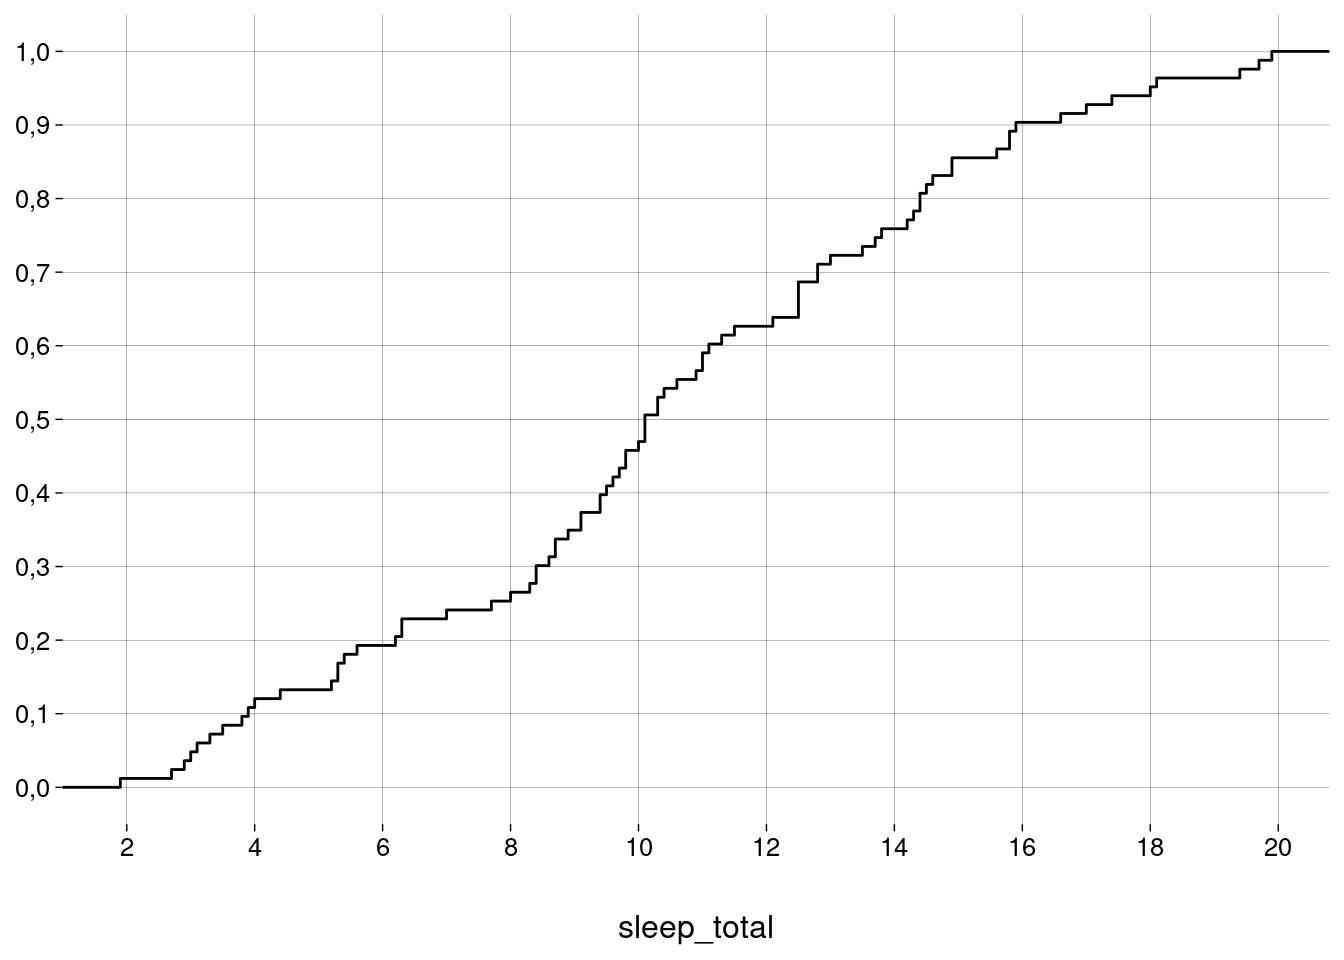
\includegraphics[width=1\linewidth]{_main_files/figure-latex/ogiva-1} \end{center}
\item
  Com a ogiva, podemos obter informações difíceis de visualizar no histograma. Por exemplo:

  \begin{itemize}
  \item
    Cerca de \(20\%\) dos mamíferos têm menos de \(6\) horas de sono.
  \item
    Cerca de metade dos mamíferos têm menos de \(10\) horas de sono.
  \item
    Cerca de \(10\%\) dos mamíferos têm mais de \(16\) horas de sono.
  \end{itemize}
\end{itemize}

\hypertarget{ramos-e-folhas}{%
\section{Ramos e folhas}\label{ramos-e-folhas}}

\begin{itemize}
\item
  No início dos anos \(1900\), quando estatísticas eram feitas à mão, Arthur Bowley criou os {\hl{diagramas de ramos e folhas}}.
\item
  Um diagrama de ramos e folhas é, basicamente, uma listagem de todos os valores de uma variável, agrupados de maneira que todos os valores de uma classe (i.e., de uma linha) têm os algarismos iniciais dentro de um intervalo.
\item
  Para as horas de sono dos mamíferos:

\begin{Shaded}
\begin{Highlighting}[]
\NormalTok{sono}\SpecialCharTok{$}\NormalTok{sleep\_total }\SpecialCharTok{\%\textgreater{}\%} 
  \FunctionTok{stem}\NormalTok{()}
\DocumentationTok{\#\# }
\DocumentationTok{\#\#   The decimal point is at the |}
\DocumentationTok{\#\# }
\DocumentationTok{\#\#    0 | 9}
\DocumentationTok{\#\#    2 | 79013589}
\DocumentationTok{\#\#    4 | 0423346}
\DocumentationTok{\#\#    6 | 23307}
\DocumentationTok{\#\#    8 | 03446779114456788}
\DocumentationTok{\#\#   10 | 01113346900135}
\DocumentationTok{\#\#   12 | 15555880578}
\DocumentationTok{\#\#   14 | 234456996889}
\DocumentationTok{\#\#   16 | 604}
\DocumentationTok{\#\#   18 | 01479}
\end{Highlighting}
\end{Shaded}
\item
  A primeira linha representa um indivíduo com \(0{,}9\) horas de sono.
\item
  A penúltima linha representa \(3\) valores:

  \begin{itemize}
  \tightlist
  \item
    \(16{,}6\)
  \item
    \(17{,}0\)
  \item
    \(17{,}4\)
  \end{itemize}
\end{itemize}

\hypertarget{exercuxedcios-3}{%
\section{Exercícios}\label{exercuxedcios-3}}

\begin{rmdimportant}
Não se esqueça de incluir títulos nos gráficos e rótulos nos eixos.

\end{rmdimportant}

\hypertarget{mamuxedferos-e-sono}{%
\subsection{Mamíferos e sono}\label{mamuxedferos-e-sono}}

\begin{rmdbox}

Use o \emph{data frame} \texttt{sono} definido como

\begin{Shaded}
\begin{Highlighting}[]
\FunctionTok{library}\NormalTok{(ggplot2)}

\NormalTok{sono }\OtherTok{\textless{}{-}}\NormalTok{ msleep }\SpecialCharTok{\%\textgreater{}\%} 
  \FunctionTok{select}\NormalTok{(}
\NormalTok{    name, order, genus, vore, bodywt, }
\NormalTok{    brainwt, awake, sleep\_total}
\NormalTok{  )}
\end{Highlighting}
\end{Shaded}

\end{rmdbox}

\begin{enumerate}
\def\labelenumi{\arabic{enumi}.}
\item
  Construa um histograma da variável \texttt{brainwt}. Escolha o número de classes que você achar melhor. O que acontece com os valores \texttt{NA}?
\item
  Descubra que função da forma \texttt{scale\_x\_...} usar para fazer com que o eixo \(x\) tenha uma escala logarítmica. Gere um novo histograma.
\item
  Qual dos dois histogramas é melhor para responder a pergunta ``\emph{Qual a faixa de peso cerebral que tem mais animais?}'' de forma satisfatória?
\item
  Construa um \emph{scatter plot} de horas de sono versus peso do cérebro. Você percebe alguma correlação entre estas variáveis? Se precisar, concentre-se em um subconjunto dos dados.
\item
  Usando \texttt{geom\_smooth} (pesquise a respeito), sobreponha uma reta de regressão ao gráfico de dispersão, usando o método \texttt{lm} e sem o erro padrão (i.e., com \texttt{se\ =\ FALSE}). O que você observa? Discuta.
\end{enumerate}

\hypertarget{igualdade-de-guxeanero-entre-furacuxf5es}{%
\subsection{Igualdade de gênero entre furacões?}\label{igualdade-de-guxeanero-entre-furacuxf5es}}

\href{https://www.pnas.org/content/111/24/8782}{Este artigo} tenta achar uma relação entre o gênero do nome de um furacão e a quantidade de vítimas fatais provocadas por ele.

\begin{rmdbox}

Os dados estão no pacote \texttt{DAAG}, que deve ser instalado:

\begin{Shaded}
\begin{Highlighting}[]
\ControlFlowTok{if}\NormalTok{ (}\SpecialCharTok{!}\FunctionTok{require}\NormalTok{(DAAG))}
  \FunctionTok{install.packages}\NormalTok{(}\StringTok{"DAAG"}\NormalTok{)}
\end{Highlighting}
\end{Shaded}

Vamos usar apenas algumas das variáveis, com nomes em português.

\begin{Shaded}
\begin{Highlighting}[]
\NormalTok{df }\OtherTok{\textless{}{-}}\NormalTok{ hurricNamed }\SpecialCharTok{\%\textgreater{}\%} 
  \FunctionTok{as\_tibble}\NormalTok{() }\SpecialCharTok{\%\textgreater{}\%} 
  \FunctionTok{transmute}\NormalTok{(}
    \AttributeTok{id =} \FunctionTok{paste}\NormalTok{(Year, Name, }\AttributeTok{sep =} \StringTok{\textquotesingle{}{-}\textquotesingle{}}\NormalTok{),}
    \AttributeTok{nome =}\NormalTok{ Name,}
    \AttributeTok{ano =}\NormalTok{ Year,}
    \AttributeTok{velocidade =}\NormalTok{ LF.WindsMPH }\SpecialCharTok{*} \FloatTok{1.8}\NormalTok{,     }\CommentTok{\# convertido para km/h}
    \AttributeTok{pressao =}\NormalTok{ LF.PressureMB,            }\CommentTok{\# mbar}
    \AttributeTok{prejuizo =}\NormalTok{ BaseDam2014 }\SpecialCharTok{\%\textgreater{}\%} \FunctionTok{round}\NormalTok{(), }\CommentTok{\# milhões de dólares de 2014}
    \AttributeTok{mortes =}\NormalTok{ deaths,}
    \AttributeTok{genero =}\NormalTok{ mf}
\NormalTok{  )}
\end{Highlighting}
\end{Shaded}

\end{rmdbox}

\begin{enumerate}
\def\labelenumi{\arabic{enumi}.}
\item
  Crie histogramas para as seguintes variáveis, escolhendo a quantidade de barras que você achar melhor.

  \begin{itemize}
  \item
    \texttt{velocidade}
  \item
    \texttt{prejuizo}
  \item
    \texttt{mortes}
  \end{itemize}

  Não se esqueça de incluir títulos nos gráficos e rótulos nos eixos.

  Comente os histogramas.
\item
  Os histogramas de prejuízos e mortes não ficaram bons. Vamos gerar histogramas transformados.

  No \emph{data frame}, crie duas novas colunas:

  \begin{itemize}
  \item
    \texttt{logprejuizo}: \emph{logaritmo} do prejuízo (na base \(10\))
  \item
    \texttt{logmortes}: \emph{logaritmo} do número de mortes (na base \(10\))
  \end{itemize}

  Agora, gere histogramas destas duas novas variáveis.
\item
  O que significa o valor do logaritmo do prejuízo na base \(10\)?
\item
  O que significa o valor do logaritmo do número de mortes na base \(10\)?
\item
  Por que o histograma do logaritmo do número de mortes vem com uma mensagem de aviso?
\item
  Por que isto não acontece com o logaritmo do prejuízo?
\item
  Faça um gráfico de dispersão com \texttt{pressao} no eixo \(y\) e \texttt{velocidade} no eixo \(x\).
\item
  Usando \texttt{geom\_smooth} (pesquise a respeito), sobreponha uma reta de regressão ao gráfico, usando o método \texttt{lm} e sem o erro padrão (i.e., com \texttt{se\ =\ FALSE}). O que você observa? Discuta.
\item
  Faça um gráfico de dispersão com \texttt{logmortes} no eixo \(y\) e \texttt{pressao} no eixo \(x\).
\item
  Usando \texttt{geom\_smooth}, sobreponha uma reta de regressão ao gráfico, usando o método \texttt{lm} e sem o erro padrão (i.e., com \texttt{se\ =\ FALSE}). O que você observa? Discuta.
\item
  Faça um gráfico de dispersão com \texttt{logmortes} no eixo \(y\) e \texttt{pressao} no eixo \(x\), com pontos coloridos de acordo com o gênero do nome do furacão.
\item
  Usando \texttt{geom\_smooth}, sobreponha retas de regressão ao gráfico, uma para cada gênero, usando o método \texttt{lm} e sem o erro padrão (i.e., com \texttt{se\ =\ FALSE}). O que você observa? Discuta.
\end{enumerate}

\begin{rmdcaution}
Visualizações como esta ajudam a explorar os dados, mas não servem para testar rigorosamente a hipótese de que furacões mulheres matam mais do que furacões homens.

Mais adiante no curso, vamos aprender a fazer testes mais rigorosos sobre hipóteses como esta.

\end{rmdcaution}

\end{document}
